\section{Đặc tả yêu cầu}
Phần này tập trung vào việc trình bày tổng quan về các chức năng chính của hệ
thống LaunchCrypt thông qua biểu đồ ca sử dụng. Mục đích chính của phần này là
giúp người đọc hiểu rõ về phạm vi, khả năng và các tương tác chính giữa người
dùng và hệ thống. Kiến thức này sẽ tạo cơ sở vững chắc để hiểu sâu hơn về cách
LaunchCrypt hoạt động và tương tác với người dùng, đồng thời cung cấp bối cảnh
cho việc đặc tả chi tiết các chức năng trong phần tiếp theo.

\subsection{Mô tả bài toán}
\hspace{1cm}Trong bối cảnh tài chính phi tập trung (DeFi) đang phát triển mạnh
mẽ, nhu cầu về một nền tảng toàn diện cho phép người dùng dễ dàng tạo, quản lý
và giao dịch token trên nhiều chuỗi khối khác nhau đang ngày càng tăng cao.
Hiện tại, việc phát hành và quản lý token trên các blockchain như Avalanche,
Solana hay Aptos vẫn đang đối mặt với nhiều thách thức về mặt kỹ thuật và hạ
tầng. Các rào cản này bao gồm yêu cầu cao về kiến thức lập trình chuyên sâu, sự
phức tạp trong quá trình triển khai hợp đồng thông minh (smart contract), cũng
như khó khăn trong việc tương tác giữa các chuỗi khối khác nhau. Đặc biệt, đối
với những doanh nghiệp nhỏ hoặc các cá nhân không có chuyên môn kỹ thuật, việc
tham gia vào hệ sinh thái token trở nên gần như bất khả thi, dẫn đến sự thiếu
cân bằng và hạn chế trong sự phát triển của hệ sinh thái Web3 nói chung.

Xuất phát từ thực trạng trên, đề tài này đề xuất phát triển một nền tảng
mang tên LaunchCrypt. Đây là một giải pháp toàn diện nhằm đơn giản hóa và
tối ưu hóa toàn bộ quy trình liên quan đến việc tạo, phân phối và giao dịch
token trên nhiều chuỗi khối khác nhau. LaunchCrypt hướng đến việc loại bỏ các
rào cản kỹ thuật hiện tại, cho phép cả người dùng chuyên nghiệp lẫn người mới
bắt đầu đều có thể dễ dàng tham gia vào hệ sinh thái token. Nền tảng này không
chỉ cung cấp công cụ để tạo token mà còn xây dựng một hệ sinh thái hoàn chỉnh,
bao gồm các tính năng giao dịch token thông qua các cặp giao dịch được tạo tự
động, khả năng gửi tiết kiệm token để sinh lợi nhuận, cũng như các tính năng
tương tác cộng đồng nhằm tăng cường trải nghiệm người dùng và tạo ra một môi
trường đầu tư lành mạnh, minh bạch.

Mục tiêu chính của LaunchCrypt là trở thành cầu nối giữa công
nghệ chuỗi khối phức tạp và nhu cầu ứng dụng thực tiễn của người dùng, từ đó
thúc đẩy quá trình phổ cập và áp dụng rộng rãi công nghệ chuỗi khối trong các
lĩnh vực khác nhau. Bằng cách cung cấp một nền tảng dễ sử dụng, an toàn và hiệu
quả, LaunchCrypt không chỉ giải quyết các vấn đề hiện tại trong hệ sinh thái
token mà còn mở ra những cơ hội mới cho sự phát triển và đổi mới trong lĩnh vực
tài chính phi tập trung, góp phần vào sự phát triển bền vững, an toàn của nền kinh tế 
số trong tương lai.

\subsection{Mô hình ca sử dụng}
\label{sec:muc2.2}
\begin{figure}[H]
    \begin{center}
        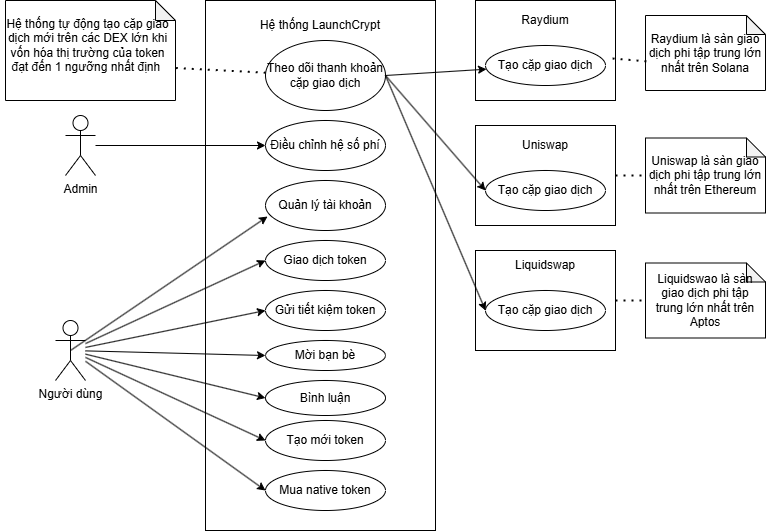
\includegraphics[width=1\textwidth]{figures/c2/UC Overall.png}
        \caption{Biểu đồ ca sử dụng tổng quát.}
        \label{fig:feature_interaction_example}
    \end{center}
\end{figure}

Các tác nhân tham gia trong biểu đồ:
\begin{description}
    \item[1.] \textbf{Người quản lý} (admin): Nắm vai trò kiểm soát hệ thống, quản
        lý hệ số phí tạo cũng như giao dịch token.

    \item[2.] \textbf{Người dùng}: Người có nhu cầu sử dụng dịch vụ của hệ thống
        LaunchCrypt.

    \item[3.] \textbf{Raydium/Liquidswap/Uniswap}: Các sàn giao dịch phi tập trung
        lớn trên các
        chuỗi khác nhau, là nơi thanh khoản sẽ được đẩy lên cho quá trình ``tốt
        nghiệp'' token.

    \item[4.] \textbf{CoinBase}: Là sàn giao dịch tập trung được dùng phổ biến,
        được sử dụng khi
        người dùng có nhu cầu mua native token của các chuối khối layer 1.
\end{description}


\begin{figure}[H]
    \begin{center}
        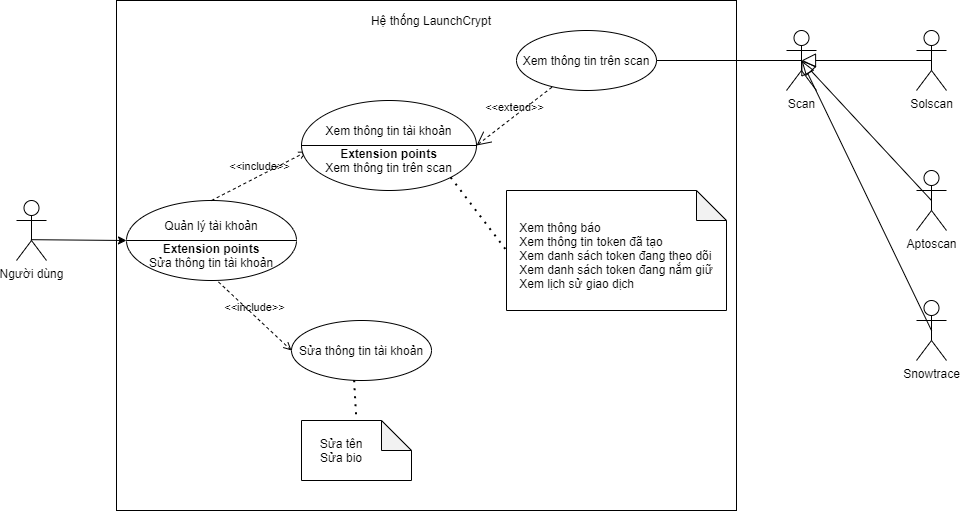
\includegraphics[width=1\textwidth]{figures/c2/User Management.png}
        \caption{Biểu đồ phân rã ca sử dụng quản lý tài khoản.}
        \label{fig:feature_interaction_example}
    \end{center}
\end{figure}
\hspace{-1cm}\textbf{Tác nhân}: Người dùng \\
\textbf{Mô tả}: Người dùng xem thông tin cá nhân và chỉnh sửa thông tin bao gồm
tên và tiểu sử (bio). Ngoài ra, người dùng có thể xem thông tin về ví của mình
trên scan.
\clearpage
\begin{figure}[H]
    \begin{center}
        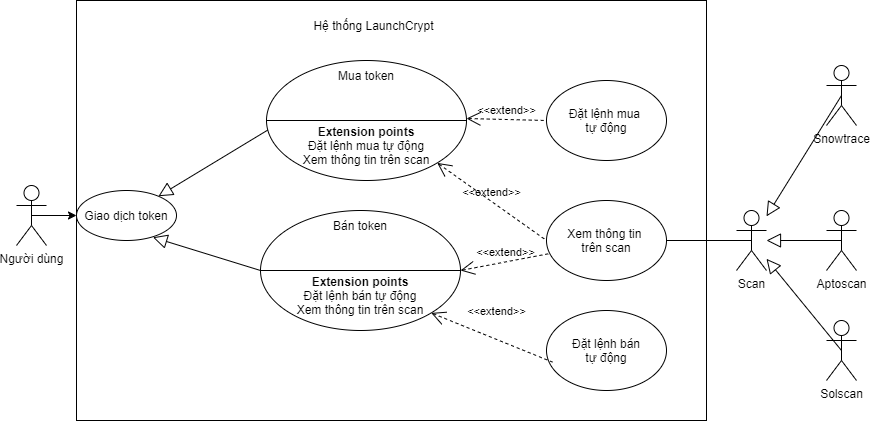
\includegraphics[width=1\textwidth]{figures/c2/TradeUCDiagram.png}
        \caption{Biểu đồ phân rã ca sử dụng giao dịch token.}
        \label{fig:feature_interaction_example}
    \end{center}
\end{figure}
\hspace{-1cm}\textbf{Tác nhân}: Người dùng \\
\textbf{Mô tả}: Người dùng giao dịch, mua bán, trao đổi giữa các token được tạo trên hệ thống và native token
trên nền tảng LaunchCrypt. Ngoài ra, người dùng có thể đặt các lệnh mua, bán tự động hoặc xem thông tin đầy đủ 
về giao dịch trên trang scan.
\clearpage

\begin{figure}[H]
    \begin{center}
        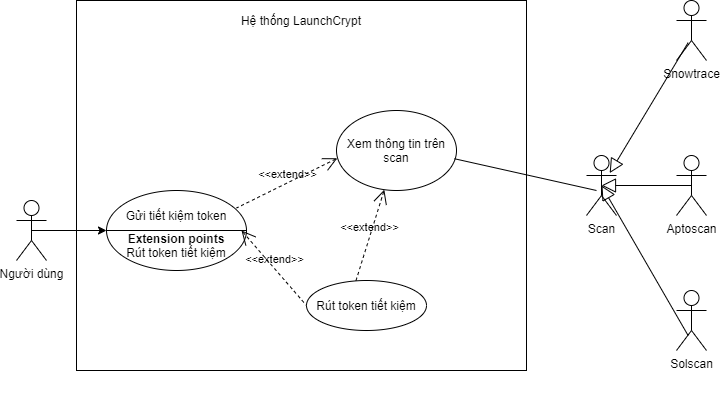
\includegraphics[width=1\textwidth]{figures/c2/GuiTKUCDiagram.png}
        \caption{Biểu đồ phân rã ca sử dụng gửi tiết kiệm token.}
        \label{fig:feature_interaction_example}
    \end{center}
\end{figure}
\hspace{-1cm}\textbf{Tác nhân}: Người dùng \\
\textbf{Mô tả}: Người dùng gửi tiết kiệm để nhận về 1 khoản lãi suất theo tỷ lệ đã quy định
trên nền tảng LaunchCrypt. Người dùng có thể rút tiền gửi tiết kiệm khi đạt đủ mốc thời gian và
xem thông tin chi tiết về các giao dịch trên trang scan.
\clearpage

\begin{figure}[H]
    \begin{center}
        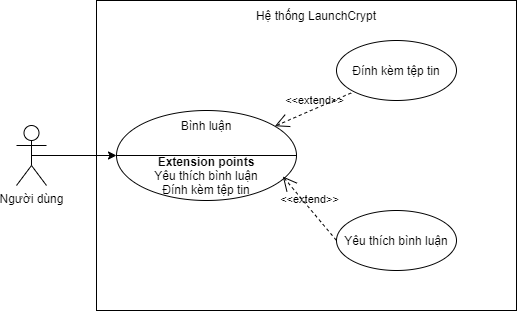
\includegraphics[width=1\textwidth]{figures/c2/Comment.png}
        \caption{Biểu đồ phân rã ca sử dụng bình luận.}
        \label{fig:feature_interaction_example}
    \end{center}
\end{figure}
\hspace{-1cm}\textbf{Tác nhân}: Người dùng \\
\textbf{Mô tả}: Khi người dùng xem thông tin giao dịch của 1 token, họ có thể
để lại bình luận hoặc trao đổi về thông tin token đó với những người dùng khác.
Người dùng cũng có thể yêu thích các bình luận, trả lời các bình luận của người
dùng khác hoặc đính kèm tệp tin trong bình luận của mình.
\clearpage

\begin{figure}[H]
    \begin{center}
        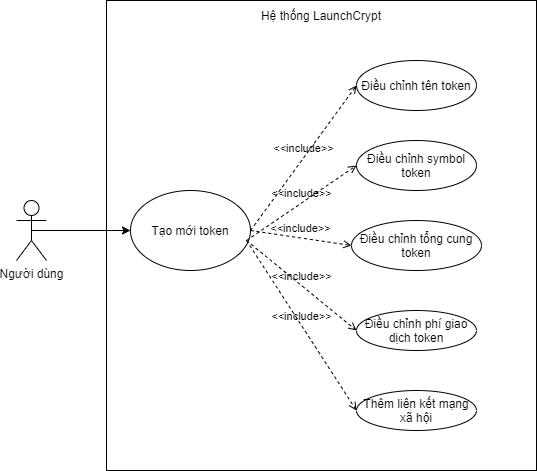
\includegraphics[width=1\textwidth]{figures/c2/CreateToken.png}
        \caption{Biểu đồ phân rã ca sử dụng tạo mới token.}
        \label{fig:feature_interaction_example}
    \end{center}
\end{figure}

\hspace{-1cm}\textbf{Tác nhân}: Người dùng \\
\textbf{Mô tả}: Người dùng tạo mới một token và điều chỉnh thông số của token
theo ý muốn. Sau khi token được tạo thành công, hệ thống LaunchCrypt sẽ tự động triển 
khai một hợp động thông minh đại diện cho cặp giao dịch giữa token này và native token.
\clearpage

\begin{figure}[H]
    \begin{center}
        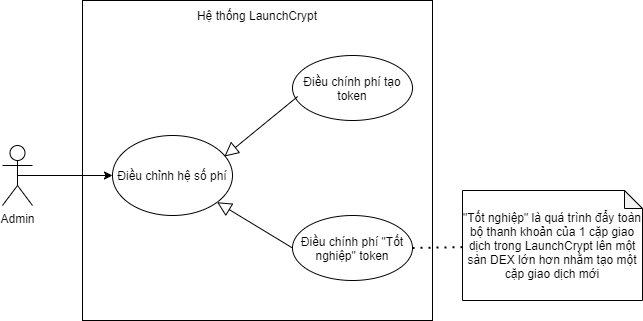
\includegraphics[width=1\textwidth]{figures/c2/FeeManagement.png}
        \caption{Biểu đồ phân rã ca sử dụng điều chỉnh hệ số phí.}
        \label{fig:feature_interaction_example}
    \end{center}
\end{figure}

\hspace{-1cm}\textbf{Tác nhân}: Admin \\
\textbf{Mô tả}: Admin điều chỉnh lượng phí mà người dùng cần trả trong quá
trình tạo và "tốt nghiệp" token.

\subsection{Đặc tả ca sử dụng}

\begin{table}[H]
    \centering
    \begin{tabular}{|p{5cm}|p{8cm}|}
        \hline
        Use case                                      & Quản lý tài khoản                                          \\
        \hline
        Tác nhân                                      & Người dùng                                                 \\
        \hline
        Tiền điều kiện                                & Người dùng đã đăng nhập thành công.                        \\
        \hline
        Hậu điều kiện                                 & Người dùng xem/cập nhật thành công thông tin tài khoản của
        mình.                                                                                                      \\
        \hline
        Luồng cơ bản                                  & 1) Người dùng lựa chọn ``Profile''. \newline
        2) Hệ thống hiển thị giao diện quản lý tài khoản với các tùy chọn. \newline
        3) Người dùng lựa chọn các mục được hiển thị trên giao diện, bao gồm:
        \begin{itemize}[leftmargin=1.5em, nosep]
            \item Xem thông báo.
            \item Xem danh sách token đang sở hữu.
            \item Xem thông tin token đã tạo.
            \item Xem danh sách token đang theo dõi.
            \item Xem danh sách user đang theo dõi.
            \item Xem danh sách token đang nắm giữ.
            \item Xem lịch sử giao dịch.
        \end{itemize}
        4) Hệ thống hiển thị thông tin tương ứng với mục mà người dùng lựa chọn.                                   \\
        \hline
        Luồng mở rộng 1: Sửa đổi thông tin tài khoản. & 3.1) Người dùng lựa chọn
        ``Edit Profile'' \newline
        4.1) Hệ thống hiển thị giao diện form sửa đổi thông tin tài khoản \newline
        5.1) Người dùng nhập thông tin vào các trường tên, bio. \newline
        6.1) Người dùng chọn ``Save Changes'' \newline
        7.1) Hệ thống hiển thị thông báo thay đổi thay công.                                                       \\
        \hline
        Luồng mở rộng 2: Xem thông tin trên scan      & 4.2) Người dùng chọn ``view
        on scan''. \newline
        5.2) Hệ thống chuyển hướng người dùng sang trang scan, hiển thị thông tin về
        tài khoản, giao dịch, ...                                                                                  \\
        \hline
    \end{tabular}
    \caption{Đặc tả ca sử dụng quản lý tài khoản.}
    \label{tab:account-management}
\end{table}

\begin{figure}[H]
    \centering
    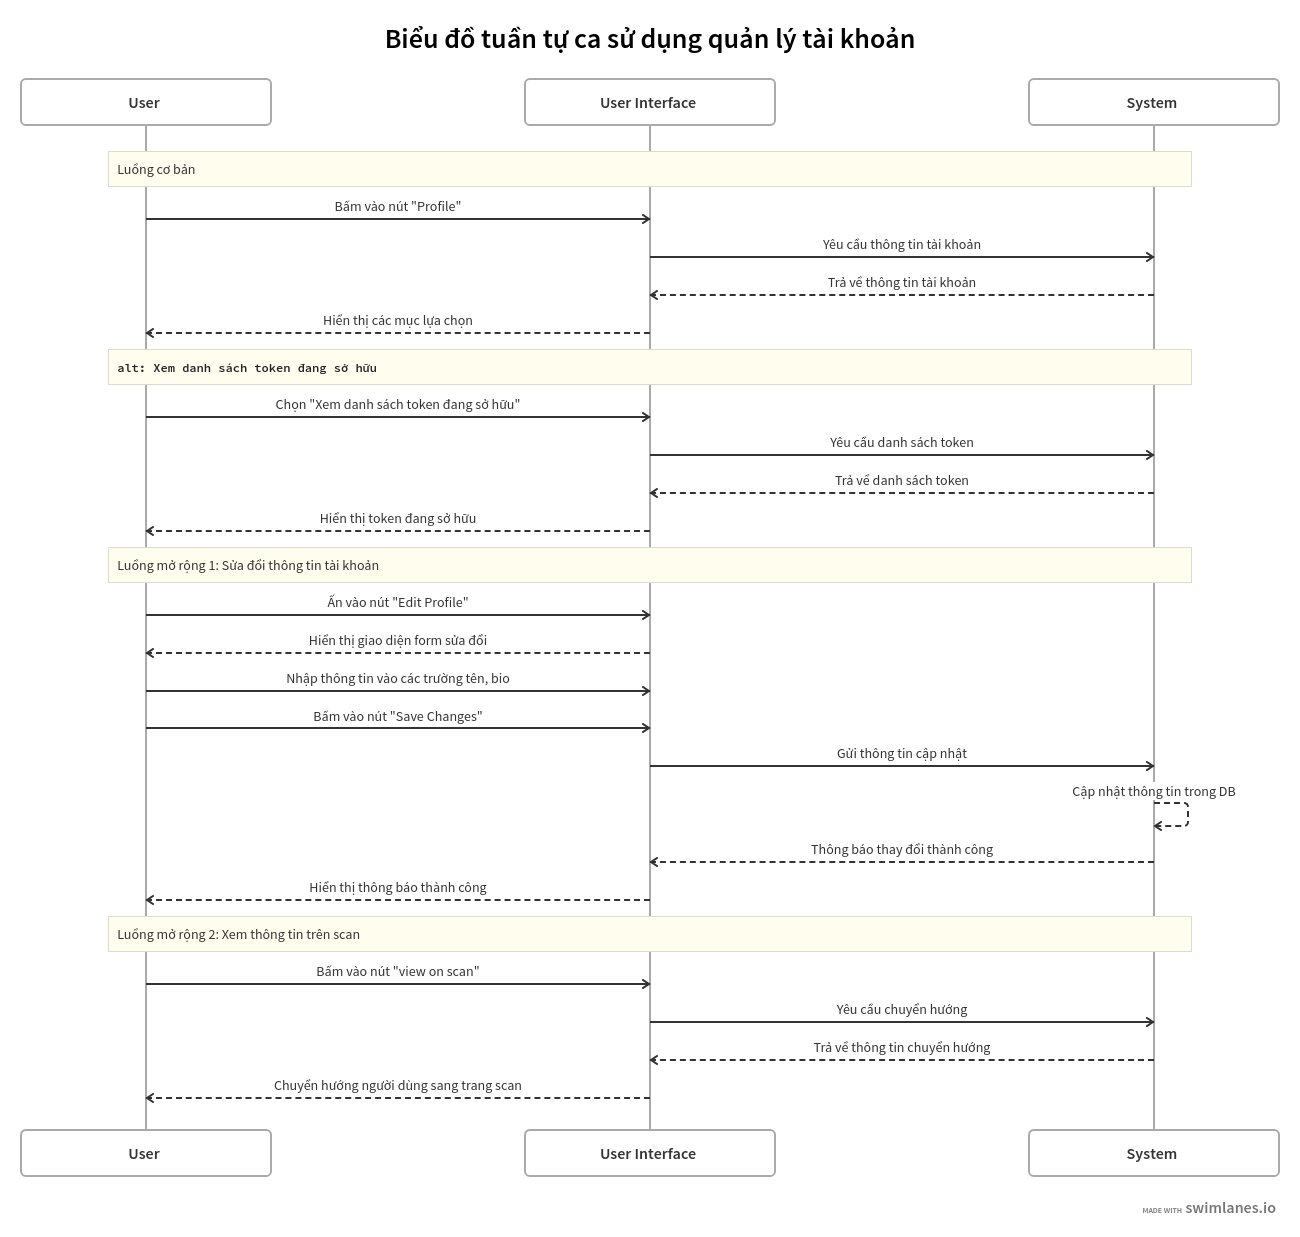
\includegraphics[width=1\textwidth]{figures/c2/ViewProfile.png}
    \caption{Biểu đồ tuần tự ca sử dụng quản lý tài khoản.}
    \label{fig:architecture-diagram}
\end{figure}

\begin{table}[H]
    \centering
    \begin{tabular}{|p{5cm}|p{8cm}|}
        \hline
        Use case                                                    & Giao dịch token                                                  \\
        \hline
        Tác nhân                                                    & Người dùng                                                       \\
        \hline
        Tiền điều kiện                                              & Người dùng đăng nhập thành công vào hệ thống.                    \\
        \hline
        Hậu điều kiện                                               & Người dùng giao dịch token thành công.                           \\
        \hline
        Luồng cơ bản                                                & 1) Người dùng tìm kiếm thông tin token, hoặc xem thông tin token
        hiển thị sẵn trên hệ thống. \newline
        2) Người dùng lựa chọn token muốn giao dịch, sau đó chọn "Trade". \newline
        3) Hệ thống hiển thị giao diện thông tin chi tiết về token. \newline
        4) Ở mục ``Buy/Sell'' trên giao diện, người dùng nhập lượng token muốn giao
        dịch. \newline
        5) Người dùng chọn ``Place trade'' \newline
        6) Hệ thống hiển thị giao diện xác nhận bao gồm thông tin về transaction, số
        token người dùng cần chi trả và số token người dùng nhận được \newline
        7) Người dùng chọn ``Confirm''. \newline
        8) Hệ thống hiển thị thông báo giao dịch thành công.                                                                           \\
        \hline
        Luồng mở rộng 1: Xem thông tin trên scan                    & 8.1) Người dùng chọn ``view on
        scan'' \newline
        9.1) Hệ thống hiển thị thông tin giao dịch trên trang scan tương ứng.                                                          \\
        \hline
        Luồng thay thế 1: Người dùng không đủ token trong tài khoản & 6.2) Hệ thống
        hiển thị thông báo lỗi, giao dịch không được thực hiện                                                                         \\
        \hline
        Luồng thay thế 2: Pool giao dịch không còn đủ token         & 6.3) Hệ thống hiển thị
        thông báo lỗi, giao dịch không được thực hiện                                                                                  \\
        \hline
    \end{tabular}
    \caption{Đặc tả ca sử dụng giao dịch token}
    \label{tab:token-transaction}
\end{table}

\begin{figure}[H]
    \centering
    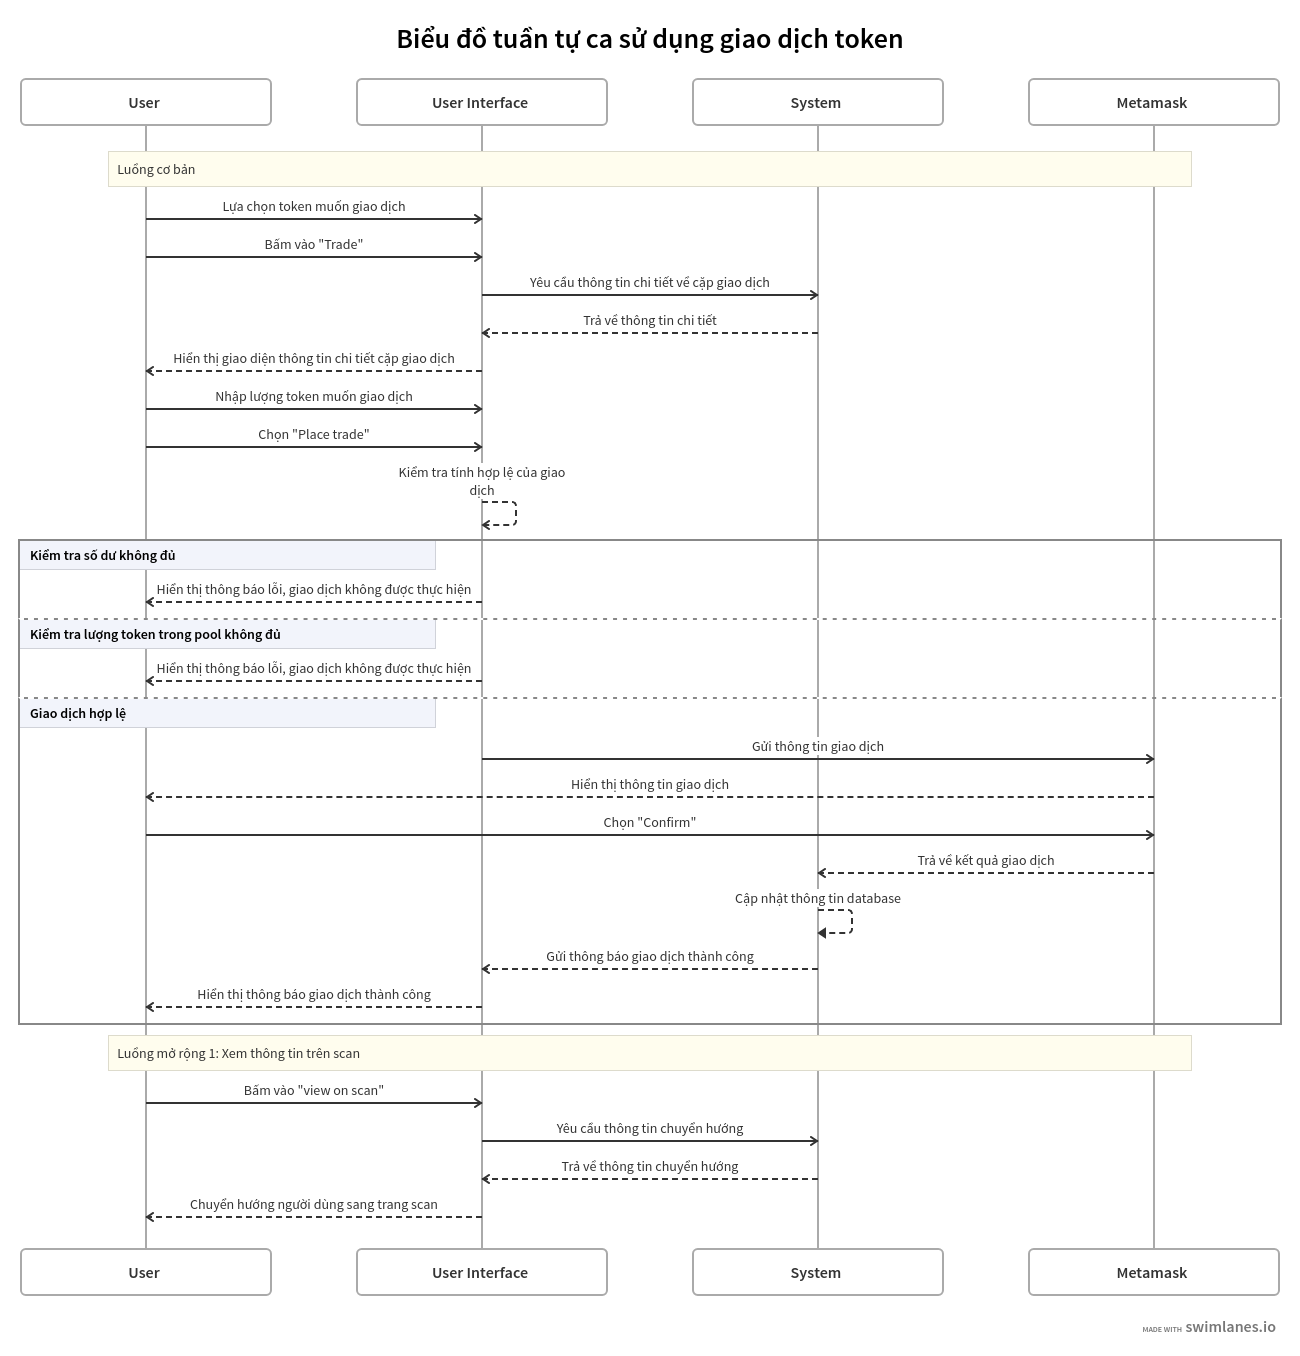
\includegraphics[width=1\textwidth]{figures/c2/TradeSeq.png}
    \caption{Biểu đồ tuần tự ca sử dụng giao dịch token.}
    \label{fig:architecture-diagram}
\end{figure}

\begin{table}[H]
    \centering
    \begin{tabular}{|p{5cm}|p{8cm}|}
        \hline
        Use case                                                        & Tự động giao dịch token                                          \\
        \hline
        Tác nhân                                                        & Người dùng                                                       \\
        \hline
        Tiền điều kiện                                                  & Người dùng đăng nhập thành công vào hệ thống.                    \\
        \hline
        Hậu điều kiện                                                   & Người dùng đặt lệnh giao dịch token thành công.                  \\
        \hline
        Luồng cơ bản                                                    & 1) Người dùng tìm kiếm thông tin token, hoặc xem thông tin token
        hiển thị sẵn trên hệ thống. \newline
        2) Người dùng lựa chọn token muốn đặt lệnh giao dịch. \newline
        3) Hệ thống hiển thị giao diện thông tin chi tiết về token. \newline
        4) Ở mục ``Order buy/sell'' trên giao diện, người dùng nhập lượng token muốn
        giao dịch, lượng native token tối đa cho lệnh (trường hợp lệnh mua) cũng như
        lượng thanh khoản cần đạt để lệnh được thực thi. \newline
        5) Người dùng chọn ``Place order'' \newline
        6) Hệ thống hiển thị giao diện xác nhận bao gồm thông tin về transaction, số
        token người dùng cần chi trả nếu lệnh được thực thi. \newline
        7) Người dùng chọn ``Confirm''. \newline
        8) Hệ thống hiển thị thông báo đặt lệnh giao dịch thành công.                                                                      \\
        \hline
        Luồng mở rộng 1: Xem thông tin trên scan                        & 8.1) Người dùng chọn ``view on
        scan'' \newline
        9.1) Hệ thống hiển thị thông tin giao dịch trên trang scan tương ứng.                                                              \\
        \hline
        Luồng thay thế 1: Người dùng không đủ token để chi trả cho lệnh & 6.3) Lệnh bị
        hủy, hệ thống hiển thị thông báo đặt lệnh không thành công.                                                                        \\
        \hline
    \end{tabular}
    \caption{Đặc tả ca sử dụng tự động đặt lệnh giao dịch token}
    \label{tab:auto-order-token}
\end{table}

\begin{figure}[H]
    \centering
    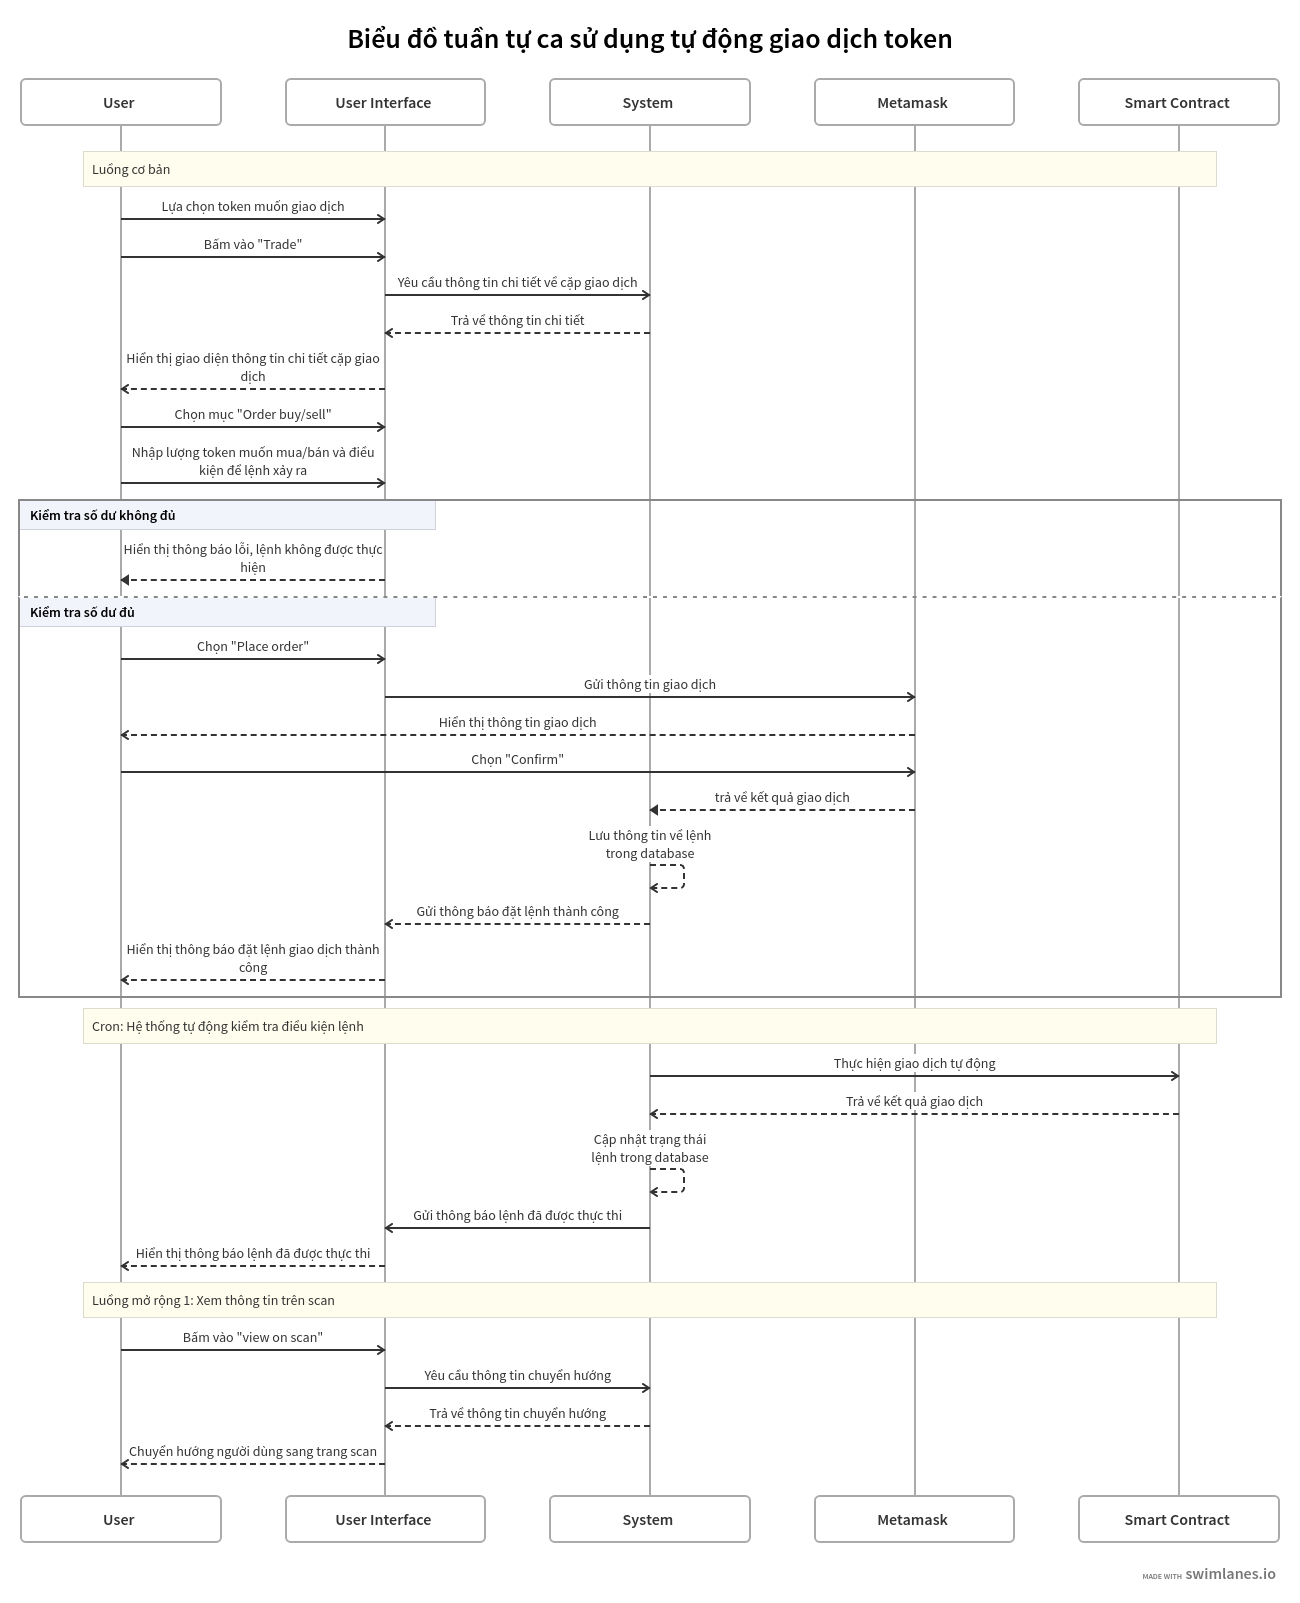
\includegraphics[width=1\textwidth]{figures/c2/AutoTradeSeq.png}
    \caption{Biểu đồ tuần tự ca sử dụng tự động giao dịch token.}
    \label{fig:architecture-diagram}
\end{figure}

\begin{table}[H]
    \centering
    \begin{tabular}{|p{5cm}|p{8cm}|}
        \hline
        Use case                                 & Gửi tiết kiệm token                                               \\
        \hline
        Tác nhân                                 & Người dùng                                                        \\
        \hline
        Tiền điều kiện                           & Người dùng đăng nhập thành công vào hệ thống.                     \\
        \hline
        Hậu điều kiện                            & Người dùng gửi tiết kiệm thành công.                              \\
        \hline
        Luồng cơ bản                             & 1) Người dùng chọn "earn" trên thanh điều hướng, sau đó
        chọn "stake". \newline
        2) Người dùng nhập lượng token muốn gửi tiết kiệm. \newline
        3) Người dùng chọn khoảng thời gian muốn gửi tiết kiệm . \newline
        4) Người dùng chọn "Stake". \newline
        5) Hệ thống hiển thị giao diện xác nhận bao gồm thông tin về transaction, số
        token người dùng cần chi trả nếu lệnh được thực thi. \newline
        6) Người dùng chọn ``Confirm''. \newline
        7) Hệ thống hiển thị thông báo gửi tiết kiệm token thành công.                                               \\
        \hline
        Luồng mở rộng 1: Rút token gửi tiết kiệm & 8.1) Người dùng chọn ``Unstake
        All''. \newline
        9.1) Hệ thống hiển thị giao diện xác nhận bao gồm thông tin về transaction, số
        token người dùng sẽ nhận được sau khi rút tiền tiết kiệm \newline
        10.1) Hệ thống hiển thị thông tin giao dịch trên trang scan tương ứng. Trong
        trường hợp người dùng chưa gửi tiết kiệm trước đó, hệ thống sẽ báo lỗi.                                      \\
        \hline
        Luồng thay thế 1: Người dùng gửi tiết kiệm khi chưa rút khoản tiền tiết kiệm cũ
        trước đó                                 & 5.2) Lệnh bị hủy, hệ thống hiển thị thông báo gửi tiết kiệm không
        thành công.                                                                                                  \\
        \hline
    \end{tabular}
    \caption{Đặc tả ca sử dụng gửi tiết kiệm token}
    \label{tab:auto-order-token}
\end{table}

\begin{figure}[H]
    \centering
    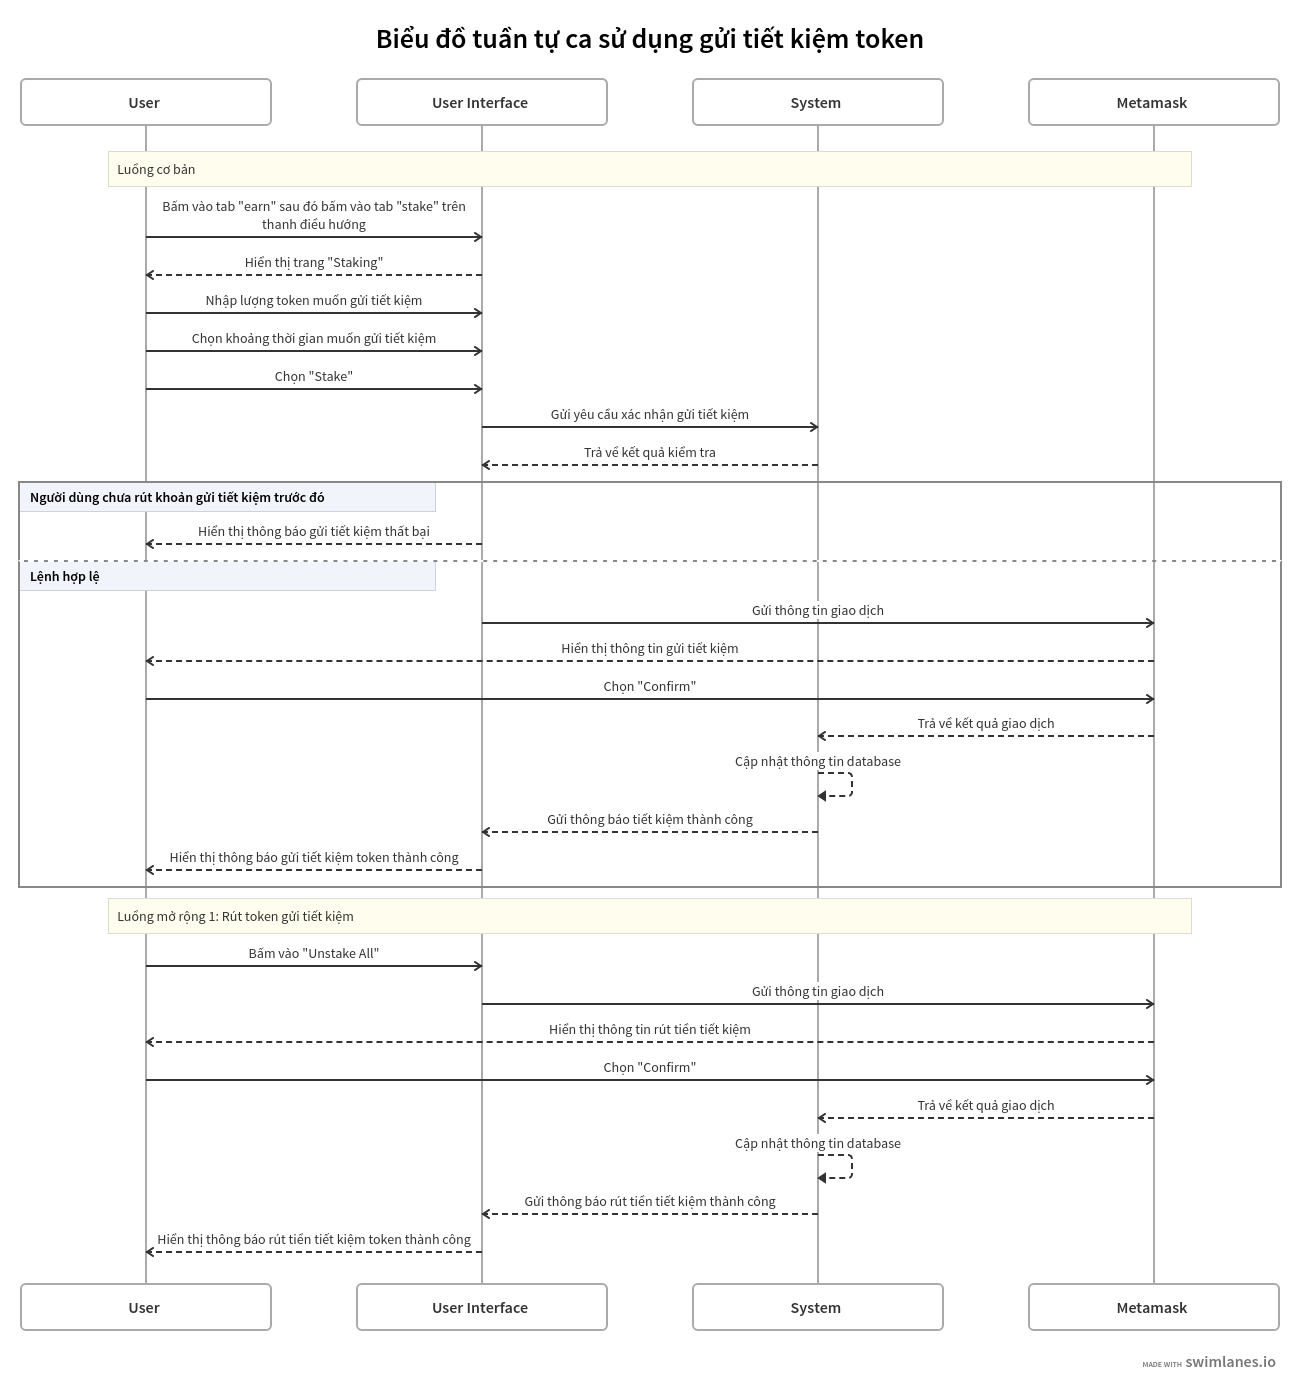
\includegraphics[width=1\textwidth]{figures/c2/StakingSeq.png}
    \caption{Biểu đồ tuần tự ca sử dụng gửi tiết kiệm token.}
    \label{fig:architecture-diagram}
\end{figure}

\begin{table}[H]
    \centering
    \begin{tabular}{|p{5cm}|p{8cm}|}
        \hline
        Use case                           & Bình luận                                                        \\
        \hline
        Tác nhân                           & Người dùng                                                       \\
        \hline
        Tiền điều kiện                     & Người dùng đăng nhập thành công vào hệ thống                     \\
        \hline
        Hậu điều kiện                      & Bình luận được đăng tải thành công                               \\
        \hline
        Luồng cơ bản                       & 1) Người dùng tìm kiếm thông tin token, hoặc xem thông tin token
        hiển thị sẵn trên hệ thống. \newline
        2) Người dùng lựa chọn token muốn xem thông tin. \newline
        3) Hệ thống hiển thị giao diện thông tin chi tiết về token. \newline
        4) Ở mục bình luận, người dùng chọn ``Post a reply'' \newline
        5) Hệ thống hiển thị hộp thông tin bao gồm nội dung comment, file đính kèm.
        \newline
        6) Người dùng nhập nội dung comment. \newline
        7) Người dùng chọn ``Send''                                                                           \\
        \hline
        Luồng mở rộng 1: Đính kèm tệp tin  & 6.1) Người dùng chọn ``Browse'' \newline
        7.1) Hệ thống hiển thị giao diện file trong máy tính của người dùng. \newline
        8.1) Người dùng chọn file muốn đăng tải. \newline
        9.1) Người dùng chọn ``Post a reply''                                                                 \\
        \hline
        Luồng mở rộng 2: Thích bình luận   & 4.2) Người dùng chọn biểu tượng trái tim cho
        bình luận mà mình thích.                                                                              \\
        \hline
        Luồng mở rộng 3: Trả lời bình luận & 4.3) Người dùng chọn bình luận mình muốn
        trả lời, chọn ``reply''                                                                                \\
        \hline
    \end{tabular}
    \caption{Đặc tả ca sử dụng bình luận}
    \label{tab:comment-usecase}
\end{table}

\begin{figure}[H]
    \centering
    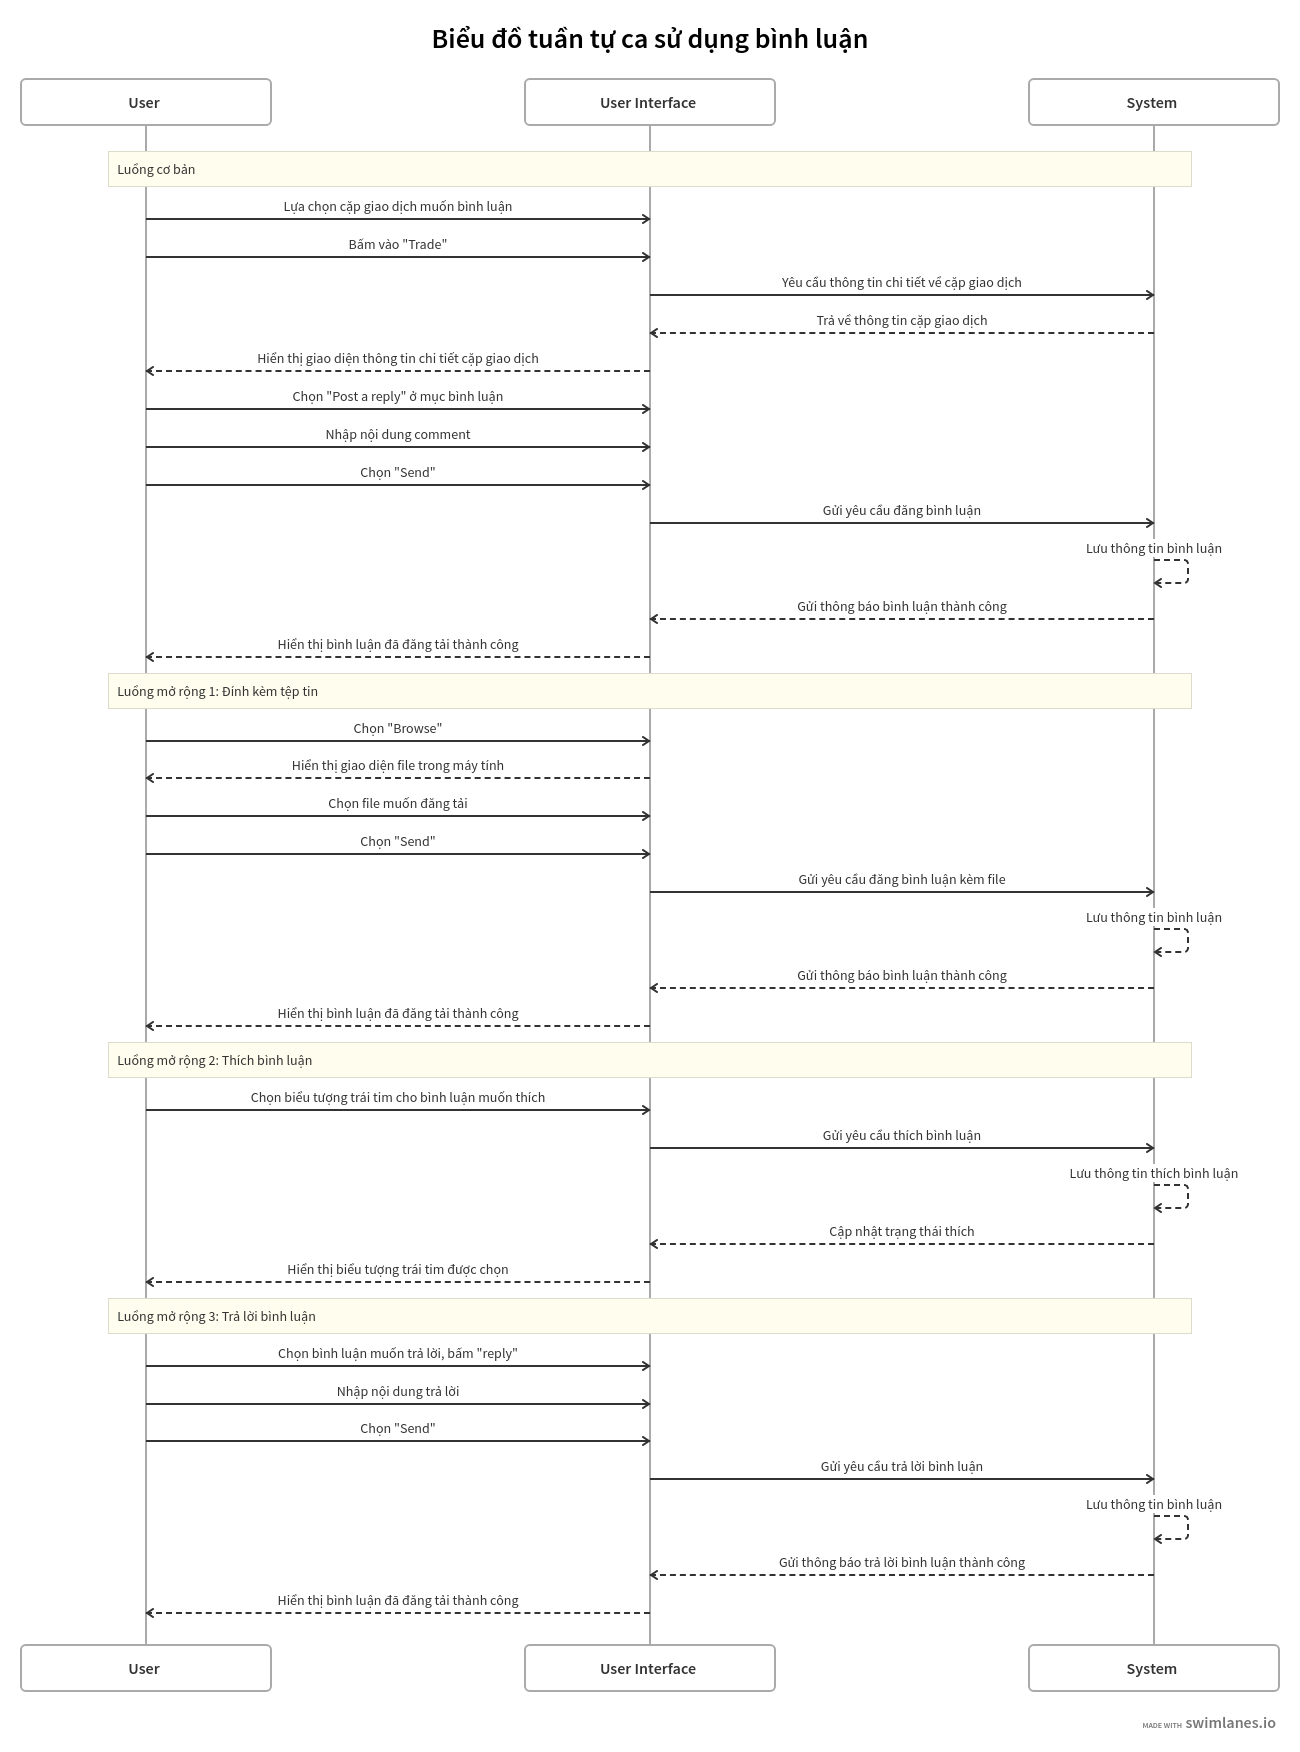
\includegraphics[width=1\textwidth]{figures/c2/CommentSeq.png}
    \caption{Biểu đồ tuần tự ca sử dụng bình luận.}
    \label{fig:architecture-diagram}
\end{figure}


\begin{table}[H]
    \centering
    \begin{tabular}{|p{5cm}|p{8cm}|}
        \hline
        Use case                                                                     & Tạo token                                    \\
        \hline
        Tác nhân                                                                     & Người dùng                                   \\
        \hline
        Tiền điều kiện                                                               & Người dùng thành công đăng nhập vào hệ thống \\
        \hline
        Hậu điều kiện                                                                & Token được tạo thành công trên hệ thống      \\
        \hline
        Luồng cơ bản                                                                 & 1) Người dùng chọn ``List token'' \newline
        2) Hệ thống hiển thị biểu mẫu bao gồm thông tin tên, ký hiệu, hình ảnh đại
        diện, description, social media link của token. \newline
        3) Người dùng điền đầy đủ thông tin token vào trong biểu mẫu, các trường thông
        tin bắt buộc bao gồm tên, ký hiệu và ảnh đại diện của token \newline
        4) Người dùng chọn ``Confirm'' \newline
        5) Hệ thống hiển thị giao diện xác nhận bao gồm thông tin về transaction,
        \newline
        6) Người dùng chọn ``Confirm''. \newline
        7) Hệ thống hiển thị thông báo tạo token thành công.                                                                        \\
        \hline
        % Luồng thay thế 1: Người dùng web2 & 5.1) Hệ thống hiển thị thông báo tạo token thành công. \\
        % \hline
        Luồng thay thế 1: Người dùng không đủ token để chi trả cho phí tạo giao dịch &
        5.1) Hệ thống hiển thị thông báo lỗi, token không được tạo thành công                                                       \\
        \hline
    \end{tabular}
    \caption{Đặc tả ca sử dụng tạo token}
    \label{tab:create-token}
\end{table}

\begin{figure}[H]
    \centering
    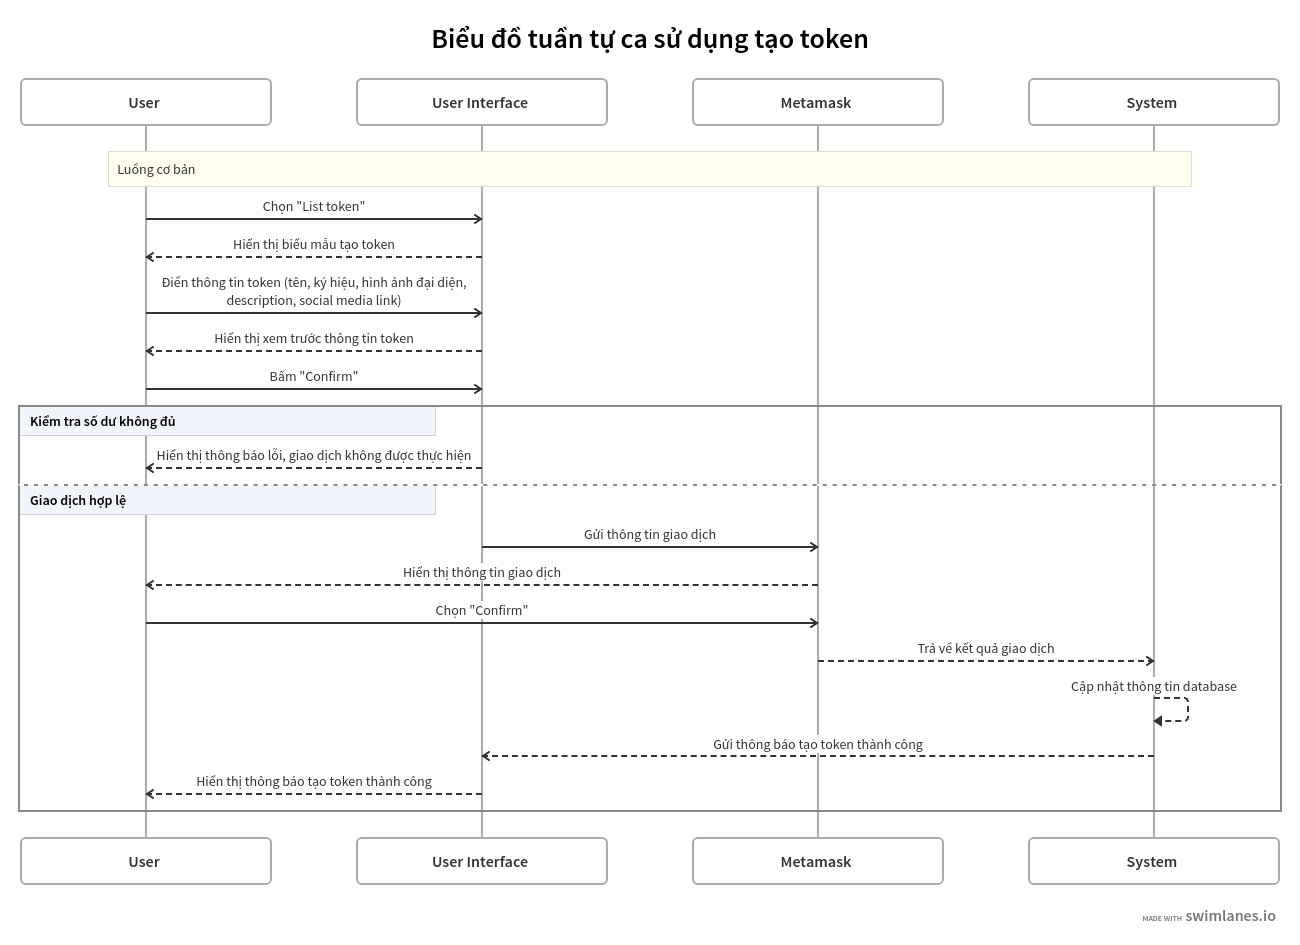
\includegraphics[width=1\textwidth]{figures/c2/TokenCreatedSeq.png}
    \caption{Biểu đồ tuần tự ca sử dụng tạo token.}
    \label{fig:architecture-diagram}
\end{figure}

\begin{table}[H]
    \centering
    \begin{tabular}{|p{5cm}|p{8cm}|}
        \hline
        Use case                                            & Điều chỉnh hệ số phí.                                      \\
        \hline
        Tác nhân                                            & Admin của hệ thống.                                        \\
        \hline
        Tiền điều kiện                                      & Admin thành công đăng nhập vào hệ thống.                   \\
        \hline
        Hậu điều kiện                                       & Hệ số phí (bao gồm chi phí tạo token, chi phí cho mỗi giao
        dịch) thay đổi theo ý muốn của admin.                                                                            \\
        \hline
        Luồng cơ bản                                        & 1) Admin ấn vào nút ``Edit Fee'' \newline
        2) Hệ thống hiển thị giao diện màn hình điều chỉnh hệ số phí. \newline
        3) Admin nhập đầy đủ thông tin các trường bao gồm chi phí tạo token, chi phí
        cho mỗi giao dịch, chuỗi khối muốn thay đổi phí. Giá trị ban đầu của hai trường
        này sẽ là giá trị đang được sử dụng. \newline
        4) Sau khi hoàn tất bước (3), Admin ấn vào nút ``Confirm''. \newline
        5) Hệ thống hiển thị thông báo thay đổi hệ số phí thành công.                                                    \\
        \hline
        Luồng thay thế 1: Không đủ token trong ví của admin & 4.1) Ví của admin không
        còn đủ token để trả phí gas \newline
        5.1) Hệ thống hiển thị thông báo thay đổi hệ số phí thất bại.                                                    \\
        \hline
    \end{tabular}
    \caption{Đặc tả ca sử dụng điều chỉnh hệ số phí.}
    \label{tab:fee-adjustment}
\end{table}

\begin{figure}[H]
    \centering
    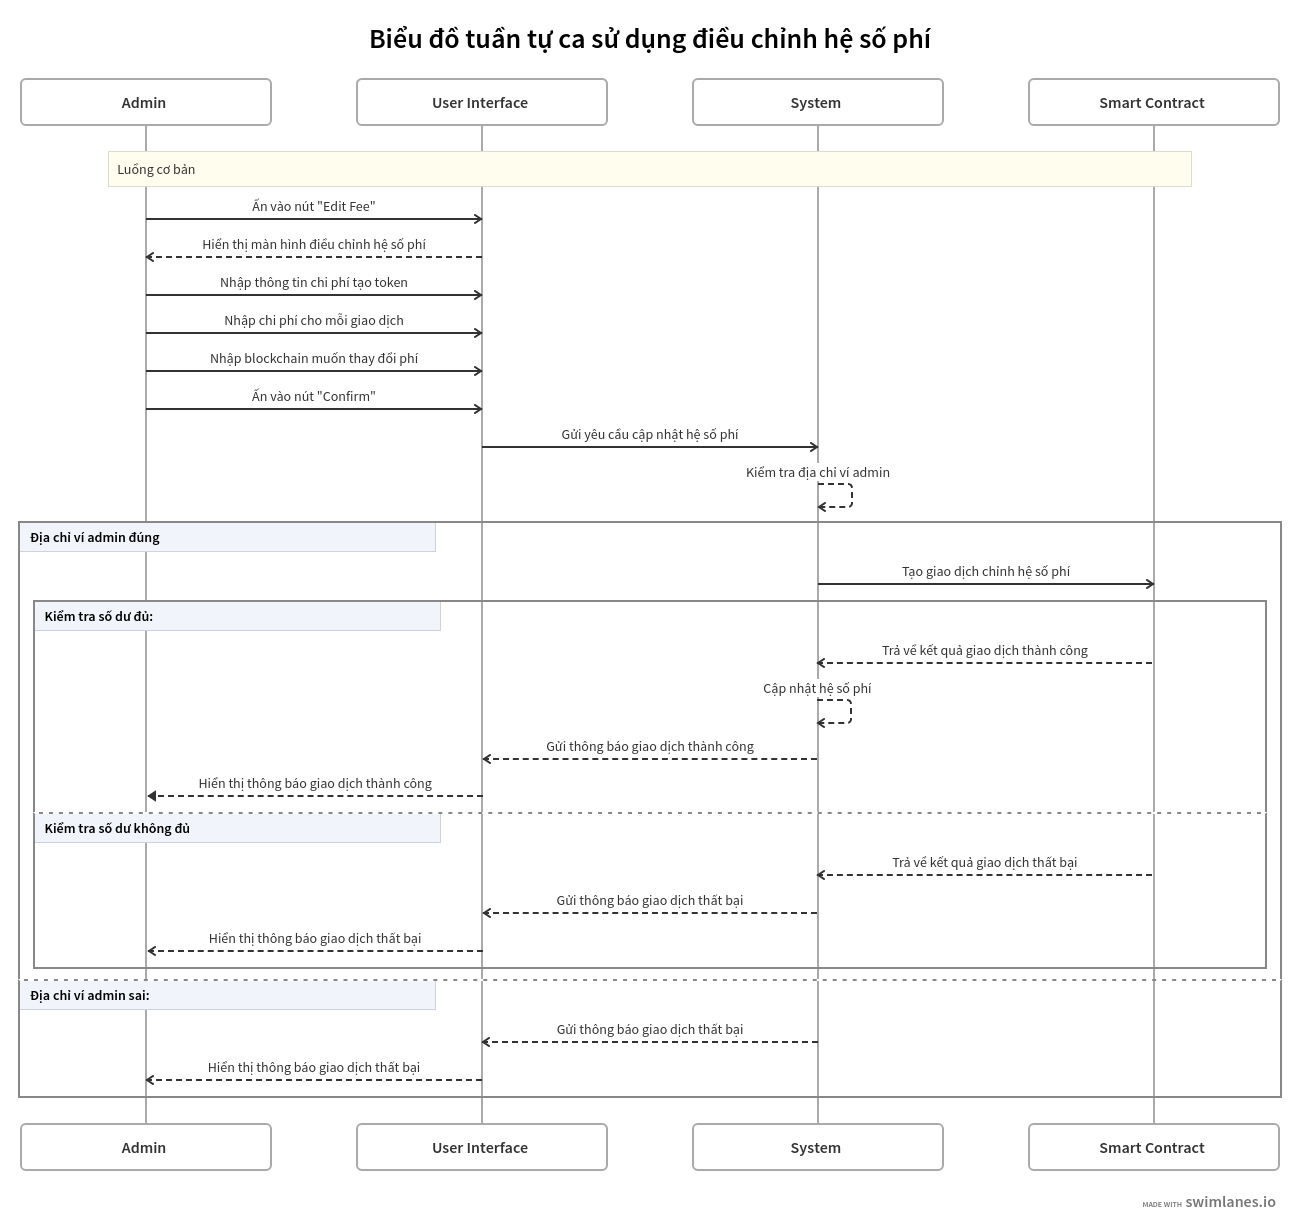
\includegraphics[width=1\textwidth]{figures/c2/ChangeFeeSeq.png}
    \caption{Biểu đồ tuần tự ca sử dụng điều chỉnh hệ số phí.}
    \label{fig:architecture-diagram}
\end{figure}

\subsection{Yêu cầu phi chức năng}
\begin{table}[H]
    \centering
    \begin{tabular}{|c|p{3cm}|p{8cm}|}
        \hline
        \textbf{STT} & \textbf{Yêu cầu}  & \textbf{Mô tả}                                               \\
        \hline
        1            & Độ trễ thấp       & Yêu cầu phần mềm có độ trễ thấp (<2 giây) để phục vụ cho nhu
        cầu giao dịch, tránh tình trạng giao dịch bị tắc hoặc bị trượt giá thường
        xuyên..                                                                                         \\
        \hline
        2            & Tính sẵn sàng     & Phần mềm cần có khả năng phục vụ các nhu cầu trong mọi thời
        điểm.                                                                                           \\
        \hline
        3            & Dữ liệu nhất quán & Đồng bộ dữ liệu được lưu trong phần mềm và các dữ liệu
        lưu trữ onchain.                                                                                \\
        \hline
        4            & Tính bảo mật      & Chi người có quyền mới được cập nhật cách hoạt động của hợp
        đồng thông minh. Ví admin phải là ví multisignature.                                            \\
        \hline
        5            & Khả năng bảo trì  & Mã nguồn được cấu trúc theo mô hình phát triển hướng
        nghiệp vụ và kiến trúc sạch (Clean architecture)                                                \\
        \hline
    \end{tabular}
    \caption{Yêu cầu phi chức năng của hệ thống}
    \label{tab:non-functional-requirements}
\end{table}

\section{Thiết kế kiến trúc}

\subsection{Tổng quan kiến trúc}

\hspace{1cm}Hệ thống được xây dựng theo mô hình 3-layer architecture, một mô
hình kiến trúc phổ biến trong phát triển phần mềm, cho phép tách biệt các thành
phần logic và dễ dàng bảo trì, mở rộng. Kiến trúc này bao gồm ba lớp chính:

\begin{description}
    \item \textbf{Presentation Layer (Controller Layer):}
          \begin{itemize}
              \item Xử lý các HTTP requests từ client
              \item Định tuyến (routing) request đến các xử lý tương ứng
              \item Validate dữ liệu đầu vào
              \item Trả về response cho client
          \end{itemize}

    \item \textbf{Business Layer (Service Layer):}
          \begin{itemize}
              \item Chứa toàn bộ business logic của ứng dụng
              \item Xử lý nghiệp vụ và các quy tắc kinh doanh
              \item Kết nối giữa Controller Layer và Data Layer
              \item Xử lý các trường hợp ngoại lệ
          \end{itemize}

    \item \textbf{Data Layer (Schema Layer):}
          \begin{itemize}
              \item Tương tác trực tiếp với cơ sở dữ liệu
              \item Định nghĩa cấu trúc dữ liệu
              \item Xử lý các thao tác CRUD với database
          \end{itemize}
\end{description}

\begin{figure}[H]
    \centering
    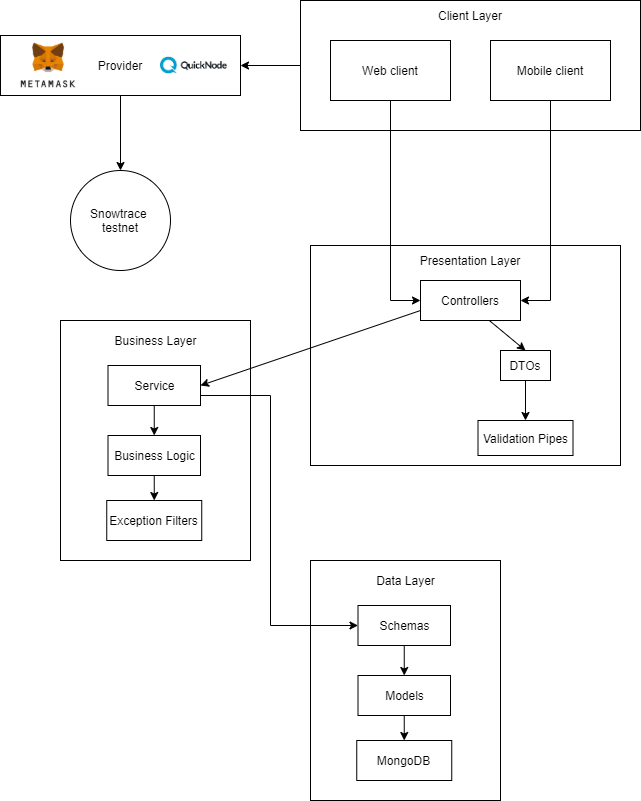
\includegraphics[width=0.8\textwidth]{figures/c2/ArchitectureOverall.png}
    \caption{Sơ đồ kiến trúc tổng quan của hệ thống.}
    \label{fig:architecture-diagram}
\end{figure}

\subsection{Điểm nổi bật của kiến trúc}

\begin{description}
    \item \textbf{Tính module hóa cao}
          \begin{itemize}
              \item Mỗi tính năng được tổ chức thành một module riêng biệt
              \item Dễ dàng phát triển và bảo trì từng module độc lập mà không cần phải
                    triển khai toàn bộ hệ thống
              \item Khả năng tái sử dụng code cao
              \item Khả năng cô lập lỗi, lỗi ở một dịch vụ sẽ không làm ngừng toàn bộ hệ
                    thống
          \end{itemize}

    \item \textbf{Dependency Injection}
          \begin{itemize}
              \item Giảm thiểu boilerplate code, từ đó làm cho mã nguồn ngắn gọn và dễ
                    bảo trì hơn
              \item Dễ dàng thay đổi implementation
              \item Thuận lợi cho việc testing
          \end{itemize}

    \item \textbf{Type Safety}
          \begin{itemize}
              \item Sử dụng TypeScript để đảm bảo type safety
              \item Giảm thiểu lỗi runtime
              \item Tăng khả năng maintain code
          \end{itemize}
\end{description}

\subsection{Chi tiết các layer}

\begin{description}
    \item \textbf{Controller Layer} \\
          Controller Layer đóng vai trò như một lớp giao tiếp giữa client và hệ thống, xử
          lý các HTTP requests và định tuyến chúng đến các xử lý tương ứng. Layer này
          được cài đặt thông qua các class được đánh dấu với decorator
          \texttt{@Controller}.

          \textbf{Cấu trúc của Controller}
          \begin{lstlisting}
@Controller('trading-pairs')
export class TradingPairsController {
   constructor(private tradingPairService: TradingPairsService) {}

   @Get()
   getAllTradingPairs(queryAllDto: QueryAllDto) {
       return this.tradingPairService.getAllTradingPairs(queryAllDto);
   }

   @Post() 
   createTradingPair(@Body() createTradingPairDto: CreateTradingPairDto) {
       return this.tradingPairService.createTradingPair(createTradingPairDto);
   }
}
\end{lstlisting}

          \textbf{Chức năng chính của Controller Layer}
          \begin{itemize}
              \item \textbf{Request Handling:} Xử lý các HTTP requests thông qua các
                    decorators như \texttt{@Get()}, \texttt{@Post()}, \texttt{@Put()},
                    \texttt{@Delete()}
              \item \textbf{Parameter Extraction:} Trích xuất dữ liệu từ request thông qua
                    các decorators \texttt{@Body()}, \texttt{@Query()}, \texttt{@Param()}
              \item \textbf{Data Validation:} Validate dữ liệu đầu vào thông qua các DTO
                    (Data Transfer Objects)
              \item \textbf{Route Management:} Quản lý các endpoints của API
          \end{itemize}

          \textbf{Validation và DTOs} \\
          \begin{lstlisting}
export class CreateTradingPairDto {
   @IsNotEmpty()
   creator: string;

   @IsNotEmpty()
   @ValidateNested({ each: true })
   @Type(() => Token)
   tokenA: Token;

   @IsNotEmpty()
   @ValidateNested({ each: true }) 
   @Type(() => Token)  
   tokenB: Token;
}
\end{lstlisting}
Data Transfer Objects (DTOs) được sử dụng để định nghĩa cấu trúc dữ liệu truyền
giữa client và server:

    \item \textbf{Service Layer} \\
          Service Layer chứa business logic của ứng dụng và đóng vai trò trung gian giữa
          Controller Layer và Data Layer. Layer này được cài đặt thông qua các class được
          đánh dấu với decorator \texttt{@Injectable()}.

          \textbf{Cấu trúc của Service}
          \begin{lstlisting}
@Injectable()
export class TradingPairsService {
   constructor(
       @InjectModel(TradingPair.name) 
       private tradingPairModel: Model<TradingPair>
   ) {}

   async getAllTradingPairs(queryAllDto: QueryAllDto): Promise<TradingPair[]> {
       const { page = 1, limit = 20, sortField, sortOrder = 'asc' } = queryAllDto;
       const skip = (page - 1) * limit;
       const sort = sortField ? 
           { [sortField]: sortOrder === 'asc' ? 1 : -1 } : {};

       return await this.tradingPairModel
           .find()
           .skip(skip)
           .limit(limit)
           .sort(sort)
           .exec();
   }
}
\end{lstlisting}

          \textbf{Chức năng chính của Service Layer}
          \begin{itemize}
              \item \textbf{Business Logic:} Xử lý các logic nghiệp vụ phức tạp
              \item \textbf{Data Transformation:} Chuyển đổi dữ liệu giữa các layer
              \item \textbf{Error Handling:} Xử lý và bắt các lỗi phát sinh
              \item \textbf{Transaction Management:} Quản lý các giao dịch với database
          \end{itemize}
\clearpage

    \item \textbf{Data Layer} \\
          Data Layer là lớp tương tác trực tiếp với cơ sở dữ liệu, được cài đặt thông qua
          các Schema và Model của Mongoose.

          \textbf{Cấu trúc của Schema}
          \begin{lstlisting}
@Schema({
   timestamps: true,
   toJSON: {
       virtuals: true,
       transform: (_, ret) => {
           delete ret._id;
           delete ret.__v;
           return ret;
       }
   }
})
export class TradingPair {
   @Prop({ required: true })
   creator: string;

   @Prop({ required: true, type: TokenSchema })
   tokenA: Token;

   @Prop({ required: true, type: TokenSchema })
   tokenB: Token;
}
\end{lstlisting}

          \textbf{Chức năng chính của Data Layer}
          \begin{itemize}
              \item \textbf{Data Definition:} Định nghĩa cấu trúc dữ liệu thông qua Schema
              \item \textbf{Data Access:} Cung cấp các phương thức truy cập dữ liệu
              \item \textbf{Data Validation:} Validate dữ liệu ở mức Schema
              \item \textbf{Query Building:} Xây dựng và thực thi các truy vấn database
          \end{itemize}
\end{description}

\section{Thiết kế chi tiết}
\subsection{Thiết kế cơ sở dữ liệu}
Từ quá trình phân tích ca sử dụng được đề cập ở mục~\ref{sec:muc2.2}, ta xác định biểu đồ thực thể liên kết và các lớp persistence như sau:

\begin{figure}[H]
    \centering
    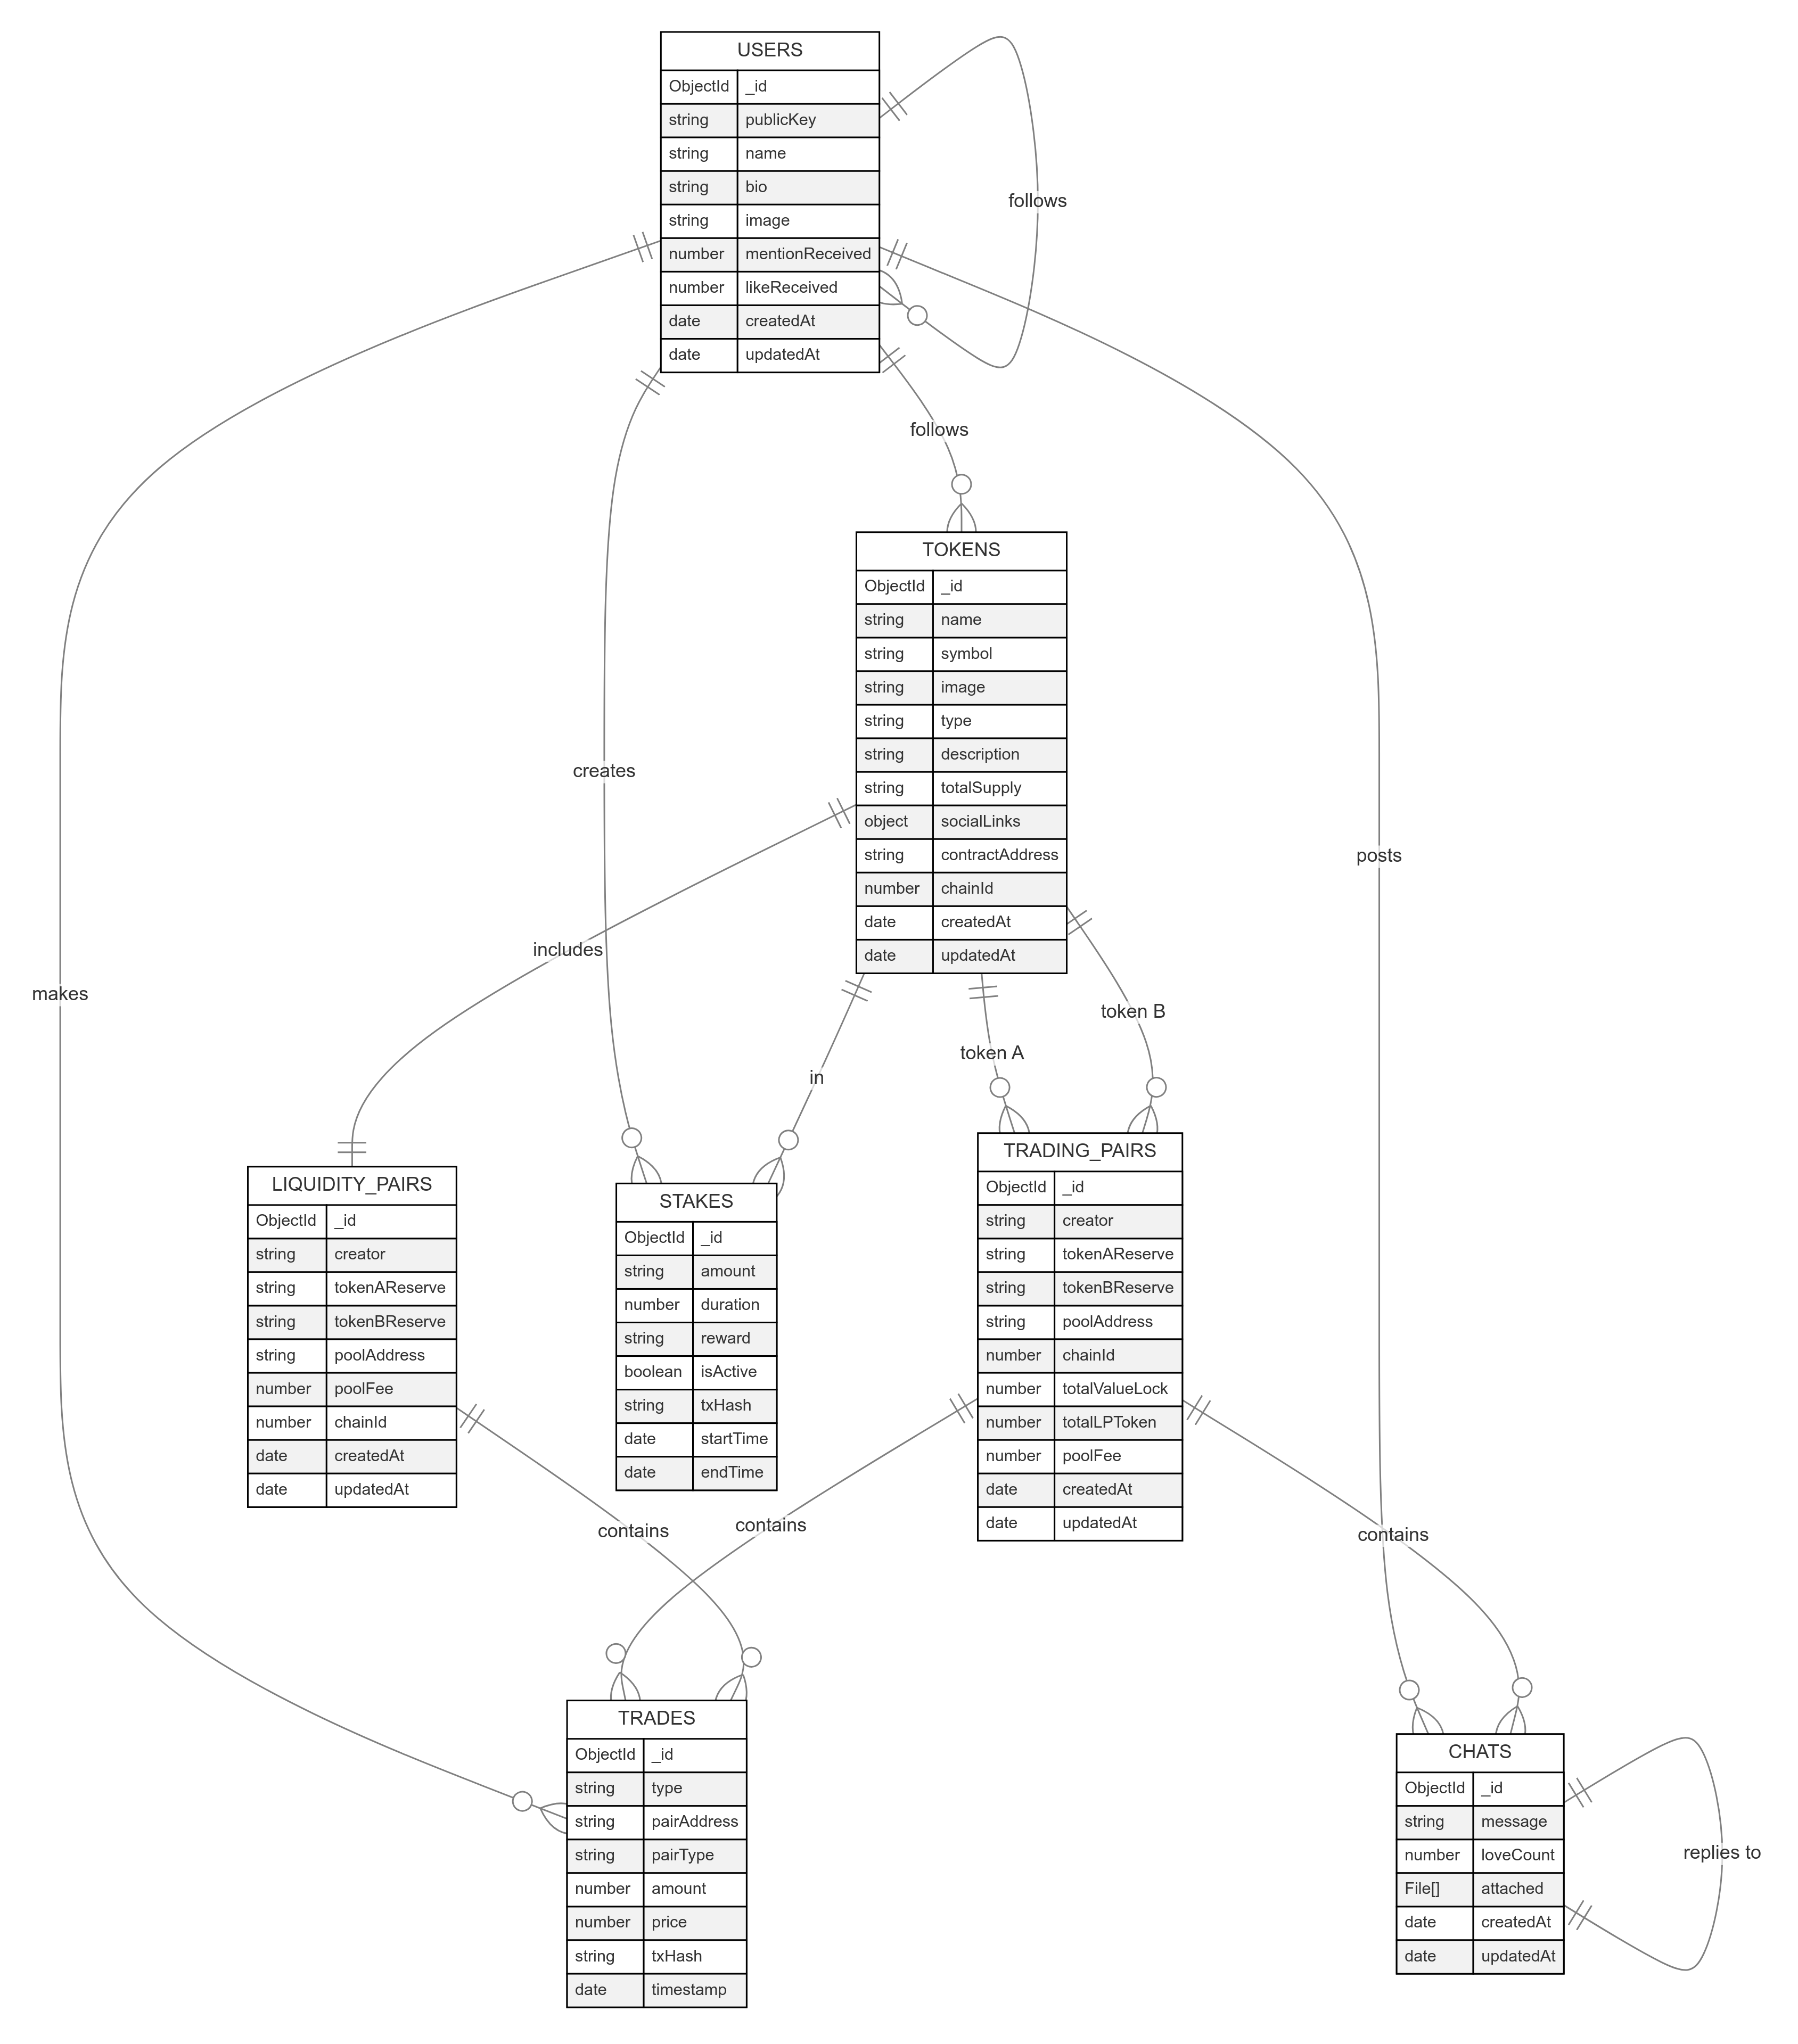
\includegraphics[width=1\textwidth]{figures/c2/DBdesign.png}
    \caption{Biểu đồ thực thể liên kết.}
    \label{fig:architecture-diagram}
\end{figure}

\begin{figure}[H]
    \centering
    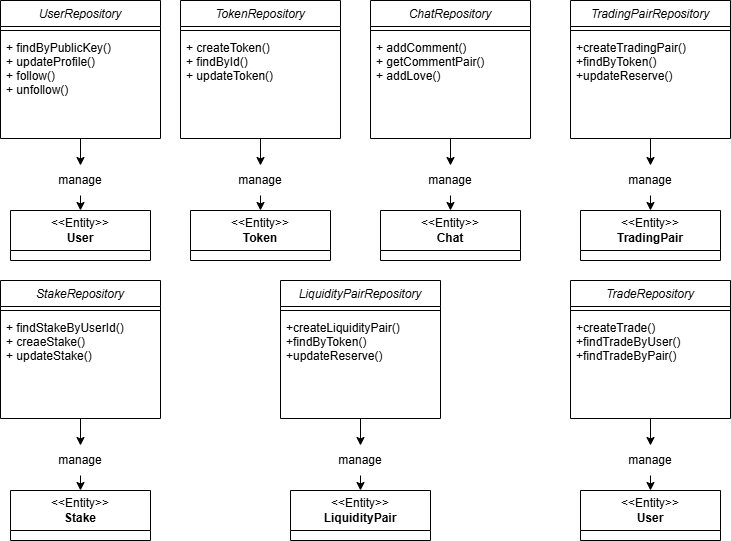
\includegraphics[width=1\textwidth]{figures/c2/persistenceClass.png}
    \caption{Biểu đồ lớp persistence.}
    \label{fig:architecture-diagram}
\end{figure}

\clearpage
\hspace{-1cm}Từ đây, ta có thiết kế các bảng trong cơ sở dữ liệu:



\hspace{-1cm}\textbf{Bảng Users}
\begin{table}[H]
    \centering
    \begin{tabular}{|c|l|l|l|}
        \hline
        STT & Thuộc tính      & Kiểu dữ liệu & Thông tin khác      \\
        \hline
        1   & id              & ObjectId     &                     \\
        \hline
        2   & publicKey       & string       &                     \\
        \hline
        3   & name            & string       &                     \\
        \hline
        4   & bio             & string       &                     \\
        \hline
        5   & follower        & objectid[]   & reference to Users  \\
        \hline
        6   & following       & objectid[]   & reference to Users  \\
        \hline
        7   & tokenFollow     & objectid[]   & reference to Tokens \\
        \hline
        8   & mentionReceived & number       &                     \\
        \hline
        9   & likeReceived    & number       &                     \\
        \hline
        10  & createdAt       & date         &                     \\
        \hline
        11  & updatedAt       & date         &                     \\
        \hline
    \end{tabular}
    \caption{Bảng Users}
    \label{tab:fee-adjustment}
\end{table}

\hspace{-1cm}\textbf{Bảng Tokens}
\begin{table}[H]
    \centering
    \begin{tabular}{|c|l|l|l|}
        \hline
        STT & Thuộc tính      & Kiểu dữ liệu & Thông tin khác \\
        \hline
        1   & id              & ObjectId     &                \\
        \hline
        2   & name            & string       &                \\
        \hline
        3   & symbol          & string       &                \\
        \hline
        4   & image           & string       &                \\
        \hline
        5   & type            & string       &                \\
        \hline
        6   & description     & string       &                \\
        \hline
        7   & totalSupply     & string       &                \\
        \hline
        8   & socialLinks     & object       &                \\
        \hline
        9   & contractAddress & string       &                \\
        \hline
        10  & chainId         & number       &                \\
        \hline
        11  & createdAt       & date         &                \\
        \hline
        12  & updatedAt       & date         &                \\
        \hline
    \end{tabular}
    \caption{Bảng Tokens}
    \label{tab:tokens}
\end{table}

\clearpage
\hspace{-1cm}\textbf{Bảng Chats}
\begin{table}[H]
    \centering
    \begin{tabular}{|c|l|l|l|}
        \hline
        STT & Thuộc tính    & Kiểu dữ liệu & Thông tin khác              \\
        \hline
        1   & id            & ObjectId     &                             \\
        \hline
        2   & creator       & string       &                             \\
        \hline
        3   & parent        & ObjectId     & reference to Chats          \\
        \hline
        4   & liquidityPair & ObjectId     & reference to LiquidityPairs \\
        \hline
        5   & message       & string       &                             \\
        \hline
        6   & loveCount     & number       &                             \\
        \hline
        7   & attached      & File[]       &                             \\
        \hline
        8   & createdAt     & date         &                             \\
        \hline
        9   & updatedAt     & date         &                             \\
        \hline
    \end{tabular}
    \caption{Bảng Chats}
    \label{tab:chats}
\end{table}

\hspace{-1cm}\textbf{Bảng Trading\_Pairs}
\begin{table}[H]
    \centering
    \begin{tabular}{|c|l|l|l|}
        \hline
        STT & Thuộc tính     & Kiểu dữ liệu & Thông tin khác      \\
        \hline
        1   & id             & ObjectId     &                     \\
        \hline
        2   & creator        & string       &                     \\
        \hline
        3   & TokenA         & ObjectId     & reference to Tokens \\
        \hline
        4   & TokenB         & ObjectId     & reference to Tokens \\
        \hline
        5   & tokenAReserve  & string       &                     \\
        \hline
        6   & tokenBReserve  & string       &                     \\
        \hline
        7   & poolAddress    & string       &                     \\
        \hline
        8   & chainId        & number       &                     \\
        \hline
        9   & totalValueLock & number       &                     \\
        \hline
        10  & totalLPToken   & number       &                     \\
        \hline
        11  & poolFee        & number       &                     \\
        \hline
        12  & createdAt      & date         &                     \\
        \hline
        13  & updatedAt      & date         &                     \\
        \hline
    \end{tabular}
    \caption{Bảng Trading\_Pairs}
    \label{tab:trading-pairs}
\end{table}

\clearpage
\hspace{-1cm}\textbf{Bảng Liquidity\_Pairs}
\begin{table}[H]
    \centering
    \begin{tabular}{|c|l|l|l|}
        \hline
        STT & Thuộc tính    & Kiểu dữ liệu & Thông tin khác      \\
        \hline
        1   & id            & ObjectId     &                     \\
        \hline
        2   & creator       & string       &                     \\
        \hline
        3   & TokenA        & ObjectId     & reference to Tokens \\
        \hline
        4   & tokenAReserve & string       &                     \\
        \hline
        5   & tokenBReserve & string       &                     \\
        \hline
        6   & poolAddress   & string       &                     \\
        \hline
        7   & poolFee       & number       &                     \\
        \hline
        8   & chainId       & number       &                     \\
        \hline
        9   & createdAt     & date         &                     \\
        \hline
        10  & updatedAt     & date         &                     \\
        \hline
    \end{tabular}
    \caption{Bảng Liquidity\_Pairs}
    \label{tab:liquidity-pairs}
\end{table}

\hspace{-1cm}\textbf{Bảng Stakes}
\begin{table}[H]
    \centering
    \begin{tabular}{|c|l|l|l|}
        \hline
        STT & Thuộc tính & Kiểu dữ liệu & Thông tin khác \\
        \hline
        1   & id         & ObjectId     &                \\
        \hline
        2   & staker     & string       &                \\
        \hline
        3   & amount     & string       &                \\
        \hline
        4   & duration   & number       &                \\
        \hline
        5   & reward     & string       &                \\
        \hline
        6   & isActive   & boolean      &                \\
        \hline
        7   & txHash     & string       &                \\
        \hline
        8   & startTime  & date         &                \\
        \hline
        9   & endTime    & date         &                \\
        \hline
    \end{tabular}
    \caption{Bảng Stakes}
    \label{tab:stakes}
\end{table}

\clearpage
\hspace{-1cm}\textbf{Bảng Trades}
\begin{table}[H]
    \centering
    \begin{tabular}{|c|l|l|l|}
        \hline
        STT & Thuộc tính  & Kiểu dữ liệu & Thông tin khác                              \\
        \hline
        1   & id          & ObjectId     &                                             \\
        \hline
        2   & type        & string       &                                             \\
        \hline
        3   & pairId      & ObjectId     & reference to LiquidityPairs || TradingPairs \\
        \hline
        4   & tokenId     & ObjectId     & reference to Tokens                         \\
        \hline
        5   & pairAddress & string       &                                             \\
        \hline
        6   & pairType    & string       &                                             \\
        \hline
        7   & amount      & number       &                                             \\
        \hline
        8   & price       & number       &                                             \\
        \hline
        9   & txHash      & string       &                                             \\
        \hline
        10  & timestamp   & date         &                                             \\
        \hline
    \end{tabular}
    \caption{Bảng Trades}
    \label{tab:trades}
\end{table}

\subsection{Thiết kế giao diện}
\begin{figure}[H]
    \centering
    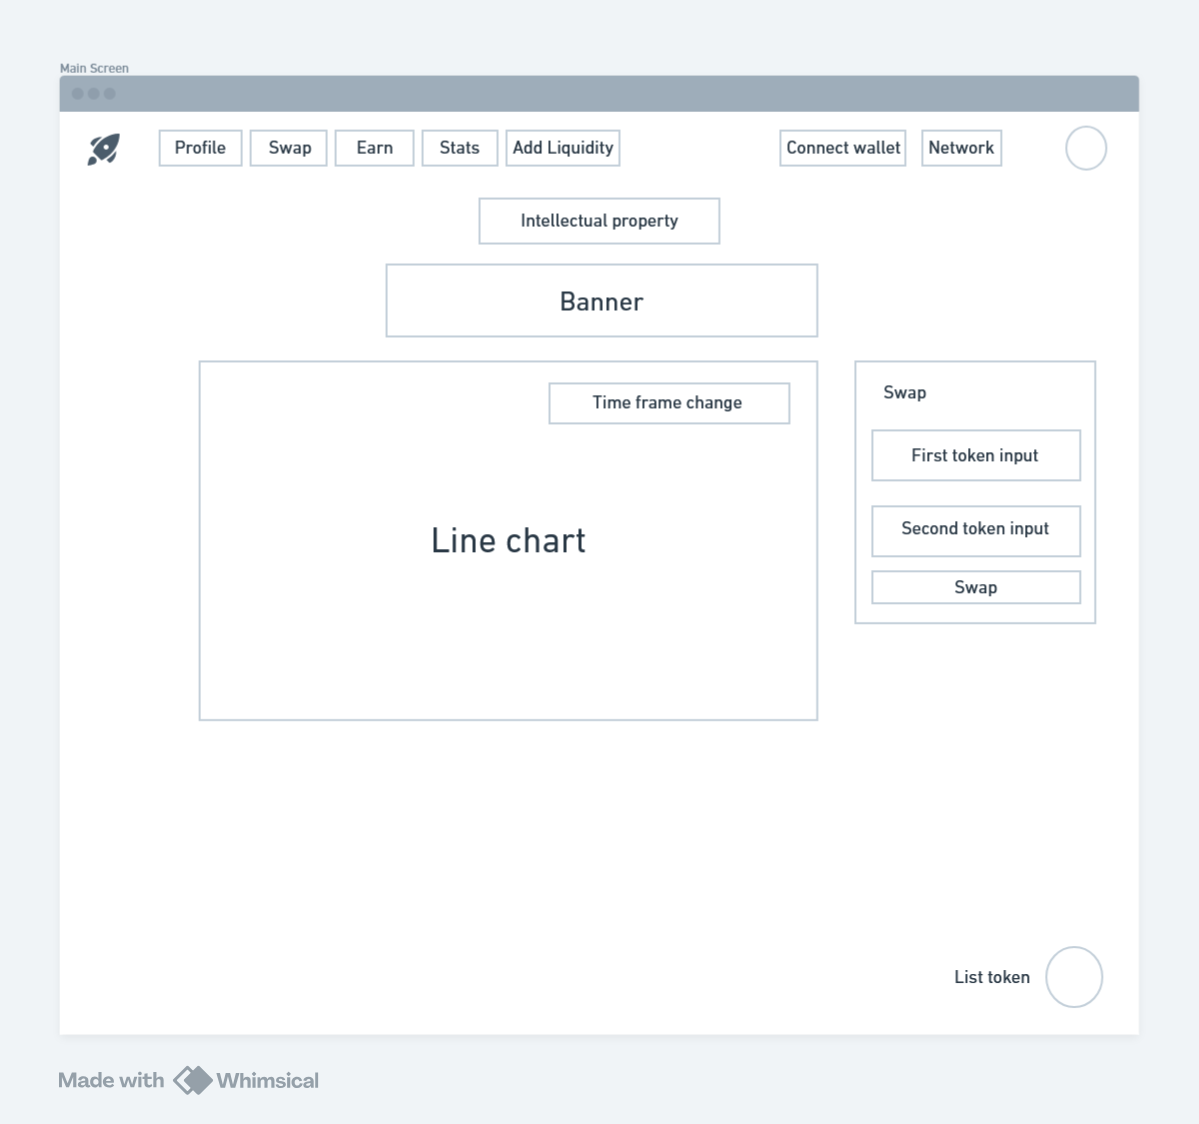
\includegraphics[width=1\textwidth]{figures/c2/MainScreen.png}
    \caption{Thiết kế trang chủ.}
    \label{fig:architecture-diagram}
\end{figure}

\begin{figure}[H]
    \centering
    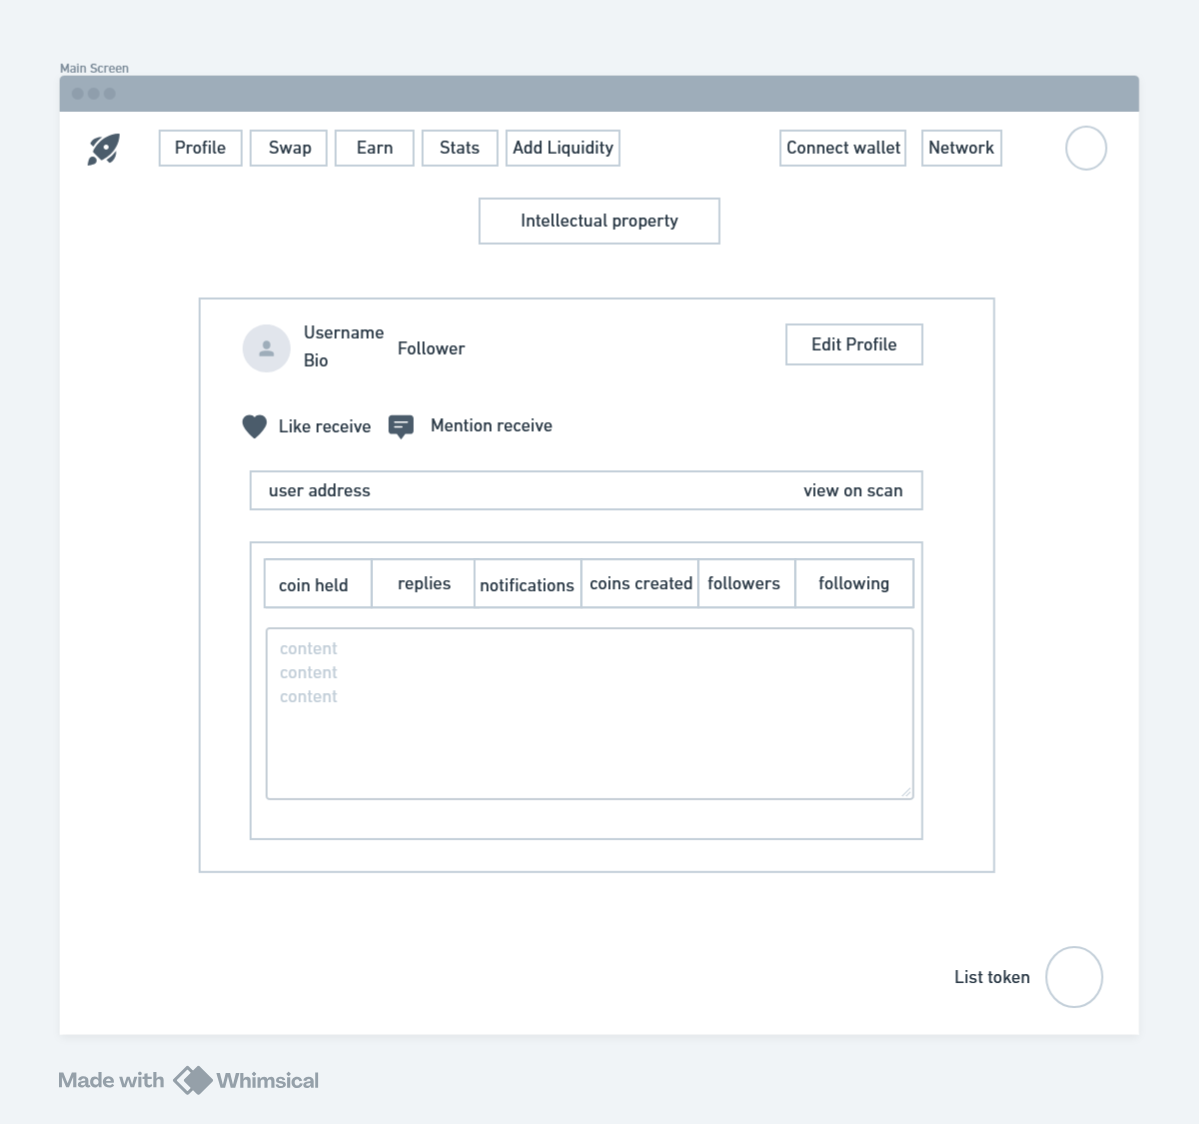
\includegraphics[width=1\textwidth]{figures/c2/Profile.png}
    \caption{Thiết kế trang thông tin người dùng.}
    \label{fig:architecture-diagram}
\end{figure}

\begin{figure}[H]
    \centering
    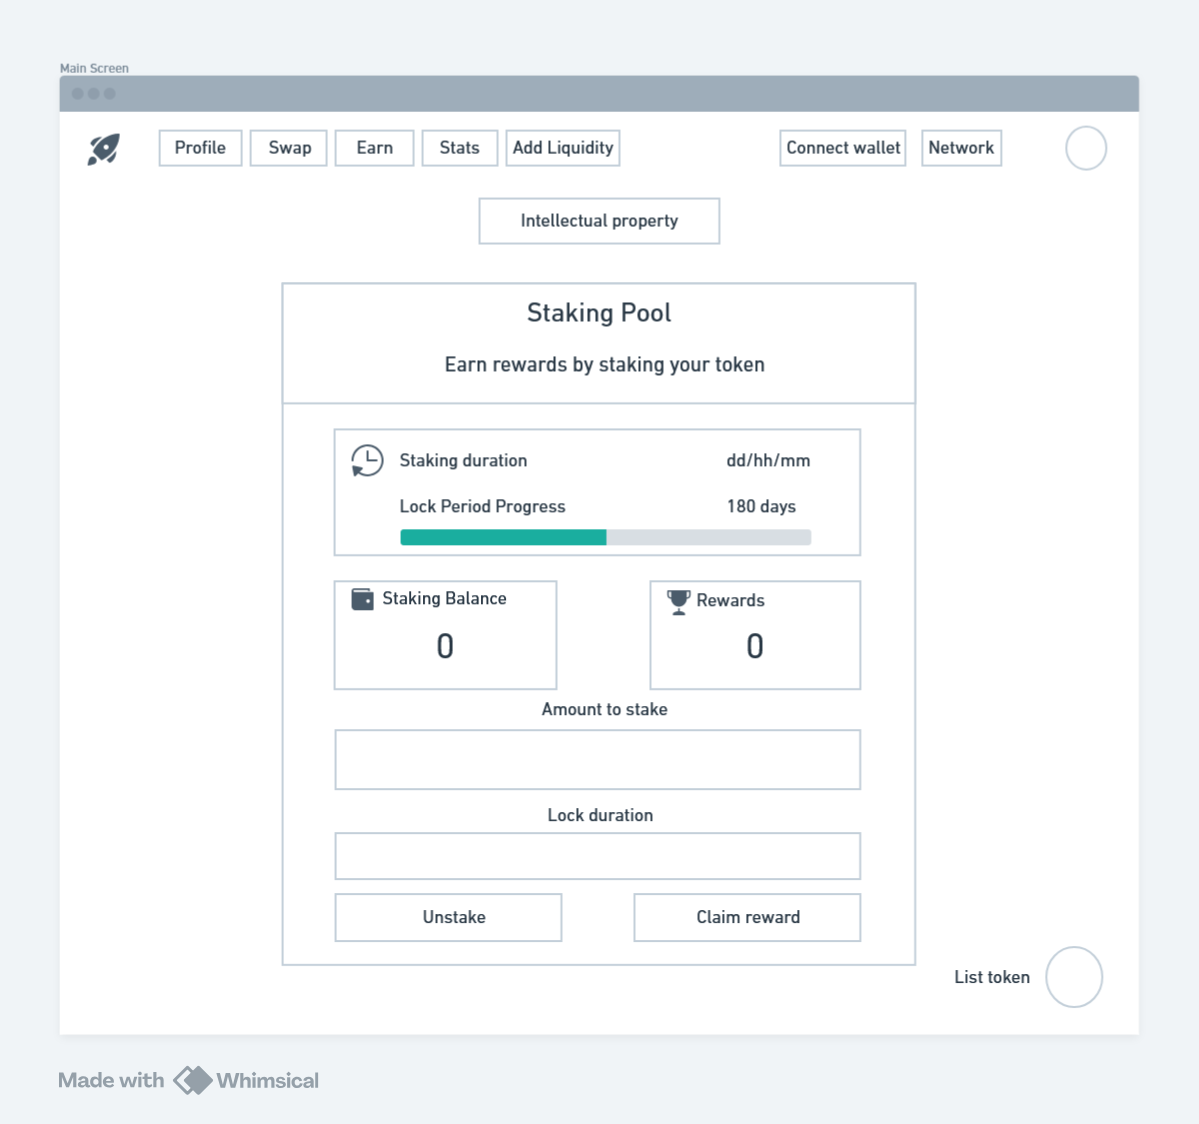
\includegraphics[width=1\textwidth]{figures/c2/Stake.png}
    \caption{Thiết kế trang gửi tiết kiệm token.}
    \label{fig:architecture-diagram}
\end{figure}

\begin{figure}[H]
    \centering
    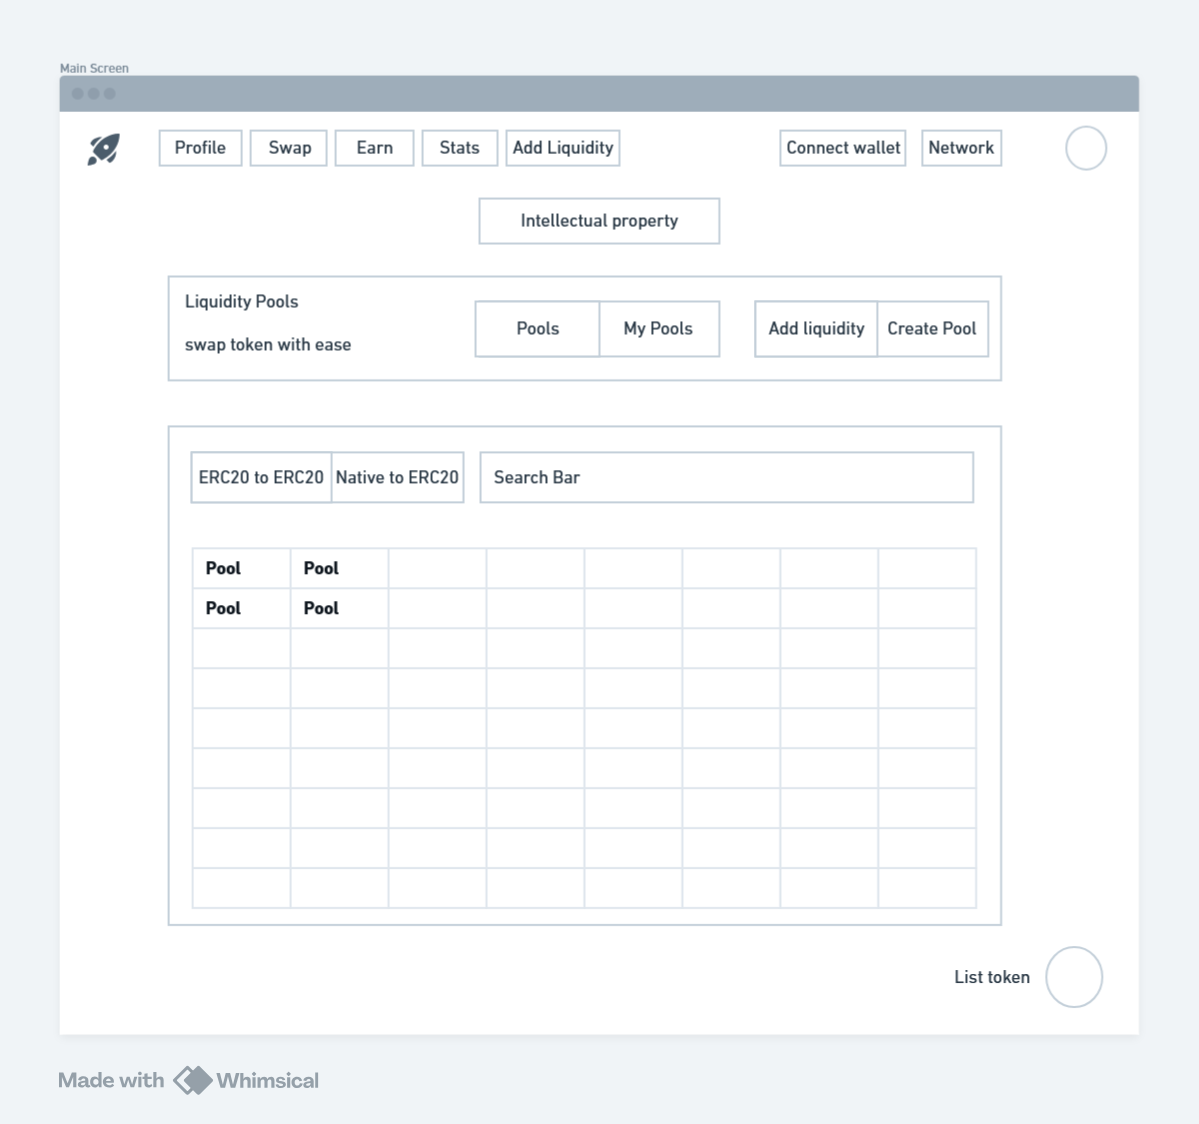
\includegraphics[width=1\textwidth]{figures/c2/Swap.png}
    \caption{Thiết kế trang hiển thị các cặp giao dịch.}
    \label{fig:architecture-diagram}
\end{figure}

\begin{figure}[H]
    \centering
    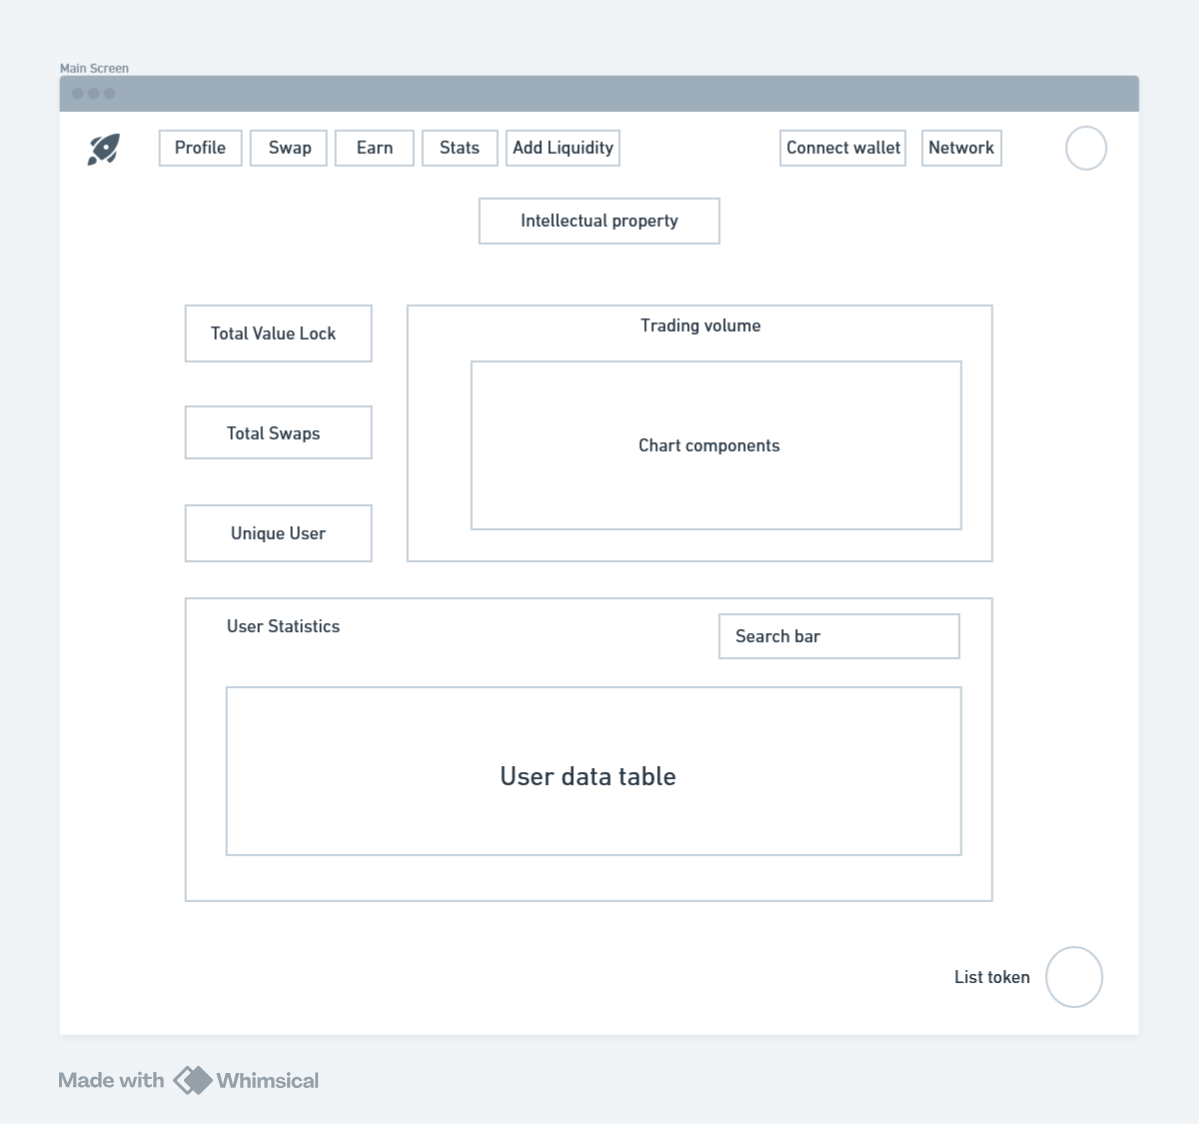
\includegraphics[width=1\textwidth]{figures/c2/Stats.png}
    \caption{Thiết kế trang thống kê thông số.}
    \label{fig:architecture-diagram}
\end{figure}

\begin{figure}[H]
    \centering
    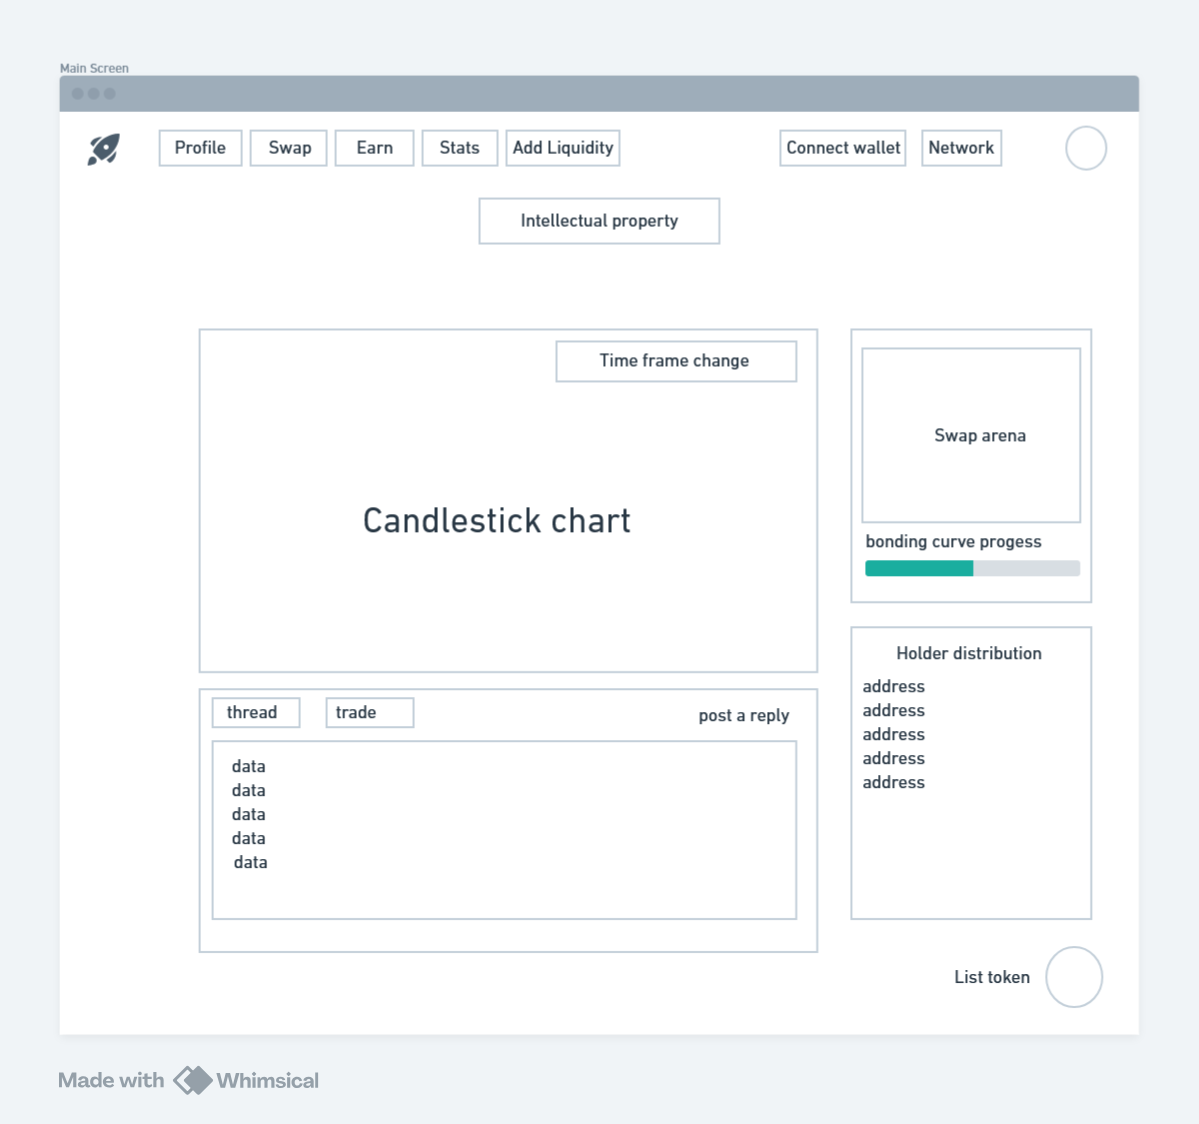
\includegraphics[width=1\textwidth]{figures/c2/Trade.png}
    \caption{Thiết kế trang giao dịch token.}
    \label{fig:architecture-diagram}
\end{figure}
